\newpage

\section{\textbf{THIẾT KẾ HỆ THỐNG}}
\subsection{\textbf{Kịch bản usecase}}
\subsubsection{Tính năng đăng ký}

\begin{table}[H]
\centering
\begin{tabular}{|l|p{11cm}|}
\hline
\textbf{Thuộc tính} & \textbf{Mô tả} \\
\hline
Use Case Name & Đăng Ký Tài Khoản (User Registration) \\
\hline
Actor & Khách (Guest User) \\
\hline
Description & Cho phép người dùng mới tạo tài khoản bằng họ tên, email và mật khẩu. Hỗ trợ đăng ký qua Google và GitHub. \\
\hline
Preconditions & 1. Người dùng chưa đăng nhập vào hệ thống \newline 2. Người dùng truy cập được trang đăng ký (/register) \newline 3. Email đăng ký chưa tồn tại trong hệ thống \\
\hline
Postconditions & 1. Tài khoản mới được tạo và lưu vào database \newline 2. Người dùng được tự động đăng nhập \newline 3. Người dùng được chuyển hướng về trang chủ \\
\hline
Normal Flow & 1. Người dùng truy cập trang đăng ký \newline 2. Nhập họ tên, email, mật khẩu, xác nhận mật khẩu \newline 3. Tick checkbox đồng ý điều khoản \newline 4. Nhấn nút "Create account" \newline 5. Hệ thống validate và tạo tài khoản \newline 6. Tự động đăng nhập và chuyển hướng về trang chủ \\
\hline
Exceptions & 1. Email đã tồn tại: Hiển thị lỗi "Email already exists" \newline 2. Mật khẩu không hợp lệ: Yêu cầu tối thiểu 6 ký tự, có chữ hoa, chữ thường, số \newline 3. Mật khẩu không khớp: Hiển thị lỗi "Passwords do not match" \newline 4. Chưa đồng ý điều khoản: Yêu cầu tick checkbox \\
\hline
\end{tabular}
\caption{Đặc tả use-case Đăng ký tài khoản}
\label{tab:uc001}
\end{table}

\subsubsection{Tính năng đăng nhập}

\begin{table}[H]
\centering
\begin{tabular}{|l|p{11cm}|}
\hline
\textbf{Thuộc tính} & \textbf{Mô tả} \\
\hline
Use Case Name & Đăng Nhập (User Login) \\
\hline
Actor & Khách (Guest User), Người dùng đã đăng ký \\
\hline
Description & Cho phép người dùng đăng nhập bằng email/mật khẩu hoặc OAuth (Google, GitHub). Hệ thống phân quyền theo vai trò USER/ADMIN. \\
\hline
Preconditions & 1. Người dùng chưa đăng nhập vào hệ thống \newline 2. Người dùng đã có tài khoản trong hệ thống \newline 3. Người dùng truy cập được trang đăng nhập (/login) \\
\hline
Postconditions & 1. Người dùng được xác thực thành công \newline 2. Access token và Refresh token được lưu vào cookies \newline 3. Người dùng được chuyển hướng đến trang phù hợp với vai trò \\
\hline
Normal Flow & 1. Người dùng truy cập trang đăng nhập \newline 2. Nhập email và mật khẩu \newline 3. Nhấn nút "Sign in" \newline 4. Hệ thống validate và xác thực thông tin \newline 5. Tạo Access Token và Refresh Token \newline 6. Lưu tokens vào cookies và chuyển hướng theo vai trò \\
\hline
Exceptions & 1. Email không tồn tại: Hiển thị lỗi "Invalid credentials" \newline 2. Mật khẩu không đúng: Hiển thị lỗi "Invalid credentials" \newline 3. Thiếu email hoặc mật khẩu: Yêu cầu điền đầy đủ thông tin \newline 4. Lỗi kết nối server: Hiển thị lỗi và yêu cầu thử lại \\
\hline
\end{tabular}
\caption{Đặc tả use-case Đăng nhập}
\label{tab:uc002}
\end{table}

\subsubsection{Tính năng bình luận sản phẩm}

\begin{table}[H]
\centering
\begin{tabular}{|l|p{11cm}|}
\hline
\textbf{Thuộc tính} & \textbf{Mô tả} \\
\hline
Use Case Name & Bình Luận Sản Phẩm (Product Comment) \\
\hline
Actor & Người dùng đã đăng nhập, Admin, Manager \\
\hline
Description & Cho phép người dùng đăng bình luận và đánh giá sản phẩm. Hệ thống tích hợp AI phân tích cảm xúc (ABSA) tự động xác định khía cạnh và cảm xúc trong bình luận. \\
\hline
Preconditions & 1. Người dùng đã đăng nhập vào hệ thống \newline 2. Sản phẩm tồn tại và đang hoạt động \newline 3. Dịch vụ AI phân tích (ML Service) khả dụng (không bắt buộc) \\
\hline
Postconditions & 1. Bình luận được lưu vào database \newline 2. AI phân tích cảm xúc và lưu kết quả (nếu thành công) \newline 3. Bình luận hiển thị trên trang sản phẩm với badge cảm xúc \\
\hline
Normal Flow & 1. Người dùng truy cập trang chi tiết sản phẩm \newline 2. Nhập nội dung bình luận (1-1000 ký tự) \newline 3. Nhấn nút "Đăng bình luận" \newline 4. Hệ thống gọi AI Service phân tích cảm xúc \newline 5. Lưu comment + aiAnalysis vào database \newline 6. Hiển thị bình luận mới với badge cảm xúc \\
\hline
Exceptions & 1. Chưa đăng nhập: Chuyển hướng đến trang login \newline 2. Nội dung rỗng: Hiển thị lỗi yêu cầu nhập nội dung \newline 3. Nội dung quá dài: Giới hạn 1000 ký tự \newline 4. AI Service không khả dụng: Lưu comment không có AI analysis \\
\hline
\end{tabular}
\caption{Đặc tả use-case Bình luận sản phẩm}
\label{tab:uc003}
\end{table}

\subsubsection{Tính năng hiển thị sản phẩm}

\begin{table}[H]
\centering
\begin{tabular}{|l|p{11cm}|}
\hline
\textbf{Thuộc tính} & \textbf{Mô tả} \\
\hline
Use Case Name & Hiển Thị Sản Phẩm (Product Listing) \\
\hline
Actor & Khách (Guest User), Người dùng đã đăng nhập \\
\hline
Description & Hiển thị danh sách sản phẩm dạng lưới với phân trang, lọc theo danh mục và sắp xếp theo nhiều tiêu chí. \\
\hline
Preconditions & 1. Hệ thống đang hoạt động và có sản phẩm trong database \newline 2. Người dùng truy cập được trang danh sách sản phẩm \\
\hline
Postconditions & 1. Danh sách sản phẩm được hiển thị đúng theo bộ lọc và thứ tự sắp xếp \newline 2. Metadata phân trang (tổng số trang, trang hiện tại) được cập nhật \newline 3. Sản phẩm hết hàng hiển thị nhãn ''Hết hàng'' \\
\hline
Normal Flow & 1. Người dùng truy cập trang danh sách sản phẩm \newline 2. Hệ thống gọi GET /api/products?page=0\&size=20 \newline 3. Hiển thị danh sách sản phẩm dạng grid với ảnh, tên, giá, rating \newline 4. Người dùng có thể lọc theo danh mục (gửi categoryId) \newline 5. Người dùng có thể sắp xếp theo giá, mới nhất, đánh giá \newline 6. Nhấn nút chuyển trang để xem thêm sản phẩm \\
\hline
Exceptions & 1. Không có sản phẩm: Hiển thị thông báo ''Không tìm thấy sản phẩm'' \newline 2. Danh mục không tồn tại: Trả về danh sách rỗng \newline 3. Tham số page vượt quá tổng số trang: Trả về trang rỗng \newline 4. Lỗi kết nối server: Hiển thị lỗi và yêu cầu thử lại \\
\hline
\end{tabular}
\caption{Đặc tả use-case Hiển thị sản phẩm}
\label{tab:uc004}
\end{table}

\subsubsection{Tính năng xem chi tiết sản phẩm}

\begin{table}[H]
\centering
\begin{tabular}{|l|p{11cm}|}
\hline
\textbf{Thuộc tính} & \textbf{Mô tả} \\
\hline
Use Case Name & Xem Chi Tiết Sản Phẩm (Product Detail) \\
\hline
Actor & Khách (Guest User), Người dùng đã đăng nhập \\
\hline
Description & Hiển thị toàn bộ thông tin chi tiết sản phẩm gồm ảnh, thông số, giá theo từng biến thể (màu sắc, dung lượng) và cho phép thêm giỏ hàng hoặc mua ngay. \\
\hline
Preconditions & 1. Sản phẩm tồn tại trong database \newline 2. Người dùng truy cập được trang chi tiết sản phẩm \\
\hline
Postconditions & 1. Thông tin sản phẩm đầy đủ được hiển thị \newline 2. Biến thể mặc định (primary variant) được chọn sẵn \newline 3. Giá và ảnh cập nhật theo biến thể đang chọn \\
\hline
Normal Flow & 1. Người dùng nhấn vào sản phẩm từ trang danh sách \newline 2. Hệ thống gọi GET /api/products/\{id\} \newline 3. Hiển thị ảnh, tên, thương hiệu, giá, thông số kỹ thuật \newline 4. Hiển thị danh sách biến thể (màu sắc, dung lượng) \newline 5. Người dùng chọn màu -- ảnh thay đổi theo variant \newline 6. Người dùng chọn dung lượng -- giá cập nhật theo variant \newline 7. Nhấn ''Thêm vào giỏ hàng'' hoặc ''Mua ngay'' \\
\hline
Exceptions & 1. Sản phẩm không tồn tại: Hiển thị lỗi 404 \newline 2. Biến thể hết hàng (stock = 0): Nút dung lượng bị mờ, không cho chọn \newline 3. Toàn bộ sản phẩm hết hàng: Vô hiệu hóa nút ''Thêm vào giỏ hàng'' \newline 4. Chưa đăng nhập khi nhấn ''Thêm vào giỏ'': Lưu vào localStorage (guest cart) \\
\hline
\end{tabular}
\caption{Đặc tả use-case Xem chi tiết sản phẩm}
\label{tab:uc005}
\end{table}

\subsubsection{Tính năng quản lý giỏ hàng}

\begin{table}[H]
\centering
\begin{tabular}{|l|p{11cm}|}
\hline
\textbf{Thuộc tính} & \textbf{Mô tả} \\
\hline
Use Case Name & Quản Lý Giỏ Hàng (Shopping Cart Management) \\
\hline
Actor & Người dùng đã đăng nhập \\
\hline
Description & Cho phép người dùng xem, thêm, cập nhật số lượng và xóa sản phẩm trong giỏ hàng. Hỗ trợ đồng bộ giỏ hàng giữa trạng thái khách và tài khoản đã đăng nhập. \\
\hline
Preconditions & 1. Người dùng đã đăng nhập vào hệ thống \newline 2. Sản phẩm muốn thêm tồn tại và còn hàng \\
\hline
Postconditions & 1. Giỏ hàng được cập nhật trên server \newline 2. Tổng tiền tạm tính được tính lại \newline 3. Số lượng giỏ hàng trên header được cập nhật \\
\hline
Normal Flow & 1. Người dùng truy cập trang giỏ hàng \newline 2. Hệ thống gọi GET /api/cart hiển thị danh sách CartItem \newline 3. Mỗi item hiển thị: ảnh, tên, biến thể, đơn giá, số lượng \newline 4. Người dùng tăng/giảm số lượng (PUT /api/cart/items/\{productId\}) \newline 5. Người dùng xóa sản phẩm (DELETE /api/cart/items/\{productId\}) \newline 6. Nhấn ''Tiến hành thanh toán'' để chuyển sang checkout \\
\hline
Exceptions & 1. Giỏ hàng rỗng: Hiển thị empty state, nút ''Tiếp tục mua sắm'' \newline 2. Số lượng vượt quá 99: Giới hạn @Max(99), hiển thị lỗi \newline 3. Số lượng nhỏ hơn 1: Giới hạn @Min(1), hiển thị lỗi \newline 4. Sản phẩm hết hàng sau khi thêm giỏ: Thông báo khi checkout \newline 5. Đăng nhập với giỏ guest: Tự động gọi POST /api/cart/sync để merge \\
\hline
\end{tabular}
\caption{Đặc tả use-case Quản lý giỏ hàng}
\label{tab:uc006}
\end{table}

\subsubsection{Tính năng đặt hàng}

\begin{table}[H]
\centering
\begin{tabular}{|l|p{11cm}|}
\hline
\textbf{Thuộc tính} & \textbf{Mô tả} \\
\hline
Use Case Name & Đặt Hàng / Thanh Toán (Place Order / Checkout) \\
\hline
Actor & Người dùng đã đăng nhập \\
\hline
Description & Cho phép người dùng nhập thông tin giao hàng, chọn phương thức thanh toán (COD/MoMo), áp dụng mã giảm giá và xác nhận đặt hàng. \\
\hline
Preconditions & 1. Người dùng đã đăng nhập vào hệ thống \newline 2. Giỏ hàng có ít nhất một sản phẩm \newline 3. Các sản phẩm trong giỏ còn hàng \\
\hline
Postconditions & 1. Đơn hàng được tạo với trạng thái PENDING \newline 2. Giỏ hàng được xóa sau khi đặt hàng thành công \newline 3. Nếu COD: paymentStatus = UNPAID; nếu MoMo: chuyển hướng sang cổng thanh toán \\
\hline
Normal Flow & 1. Nhấn ''Tiến hành thanh toán'' từ giỏ hàng \newline 2. Nhập thông tin giao hàng: email, họ tên, SĐT, địa chỉ đầy đủ \newline 3. Chọn phương thức thanh toán: COD hoặc MoMo \newline 4. Nhập mã giảm giá sản phẩm/vận chuyển (tùy chọn) \newline 5. Xem tóm tắt đơn hàng và nhấn ''Đặt hàng'' \newline 6. Hệ thống tạo đơn, chuyển đến trang đặt hàng thành công \\
\hline
Exceptions & 1. Thiếu thông tin bắt buộc: Hiển thị lỗi validation \newline 2. Mã voucher không hợp lệ hoặc hết hạn: Hiển thị lỗi \newline 3. Sản phẩm hết hàng khi đặt: Yêu cầu cập nhật giỏ hàng \newline 4. Nhấn đặt hàng nhiều lần: idempotencyKey ngăn tạo đơn trùng \\
\hline
\end{tabular}
\caption{Đặc tả use-case Đặt hàng}
\label{tab:uc007}
\end{table}

\subsubsection{Tính năng yêu thích sản phẩm}

\begin{table}[H]
\centering
\begin{tabular}{|l|p{11cm}|}
\hline
\textbf{Thuộc tính} & \textbf{Mô tả} \\
\hline
Use Case Name & Yêu Thích Sản Phẩm (Wishlist) \\
\hline
Actor & Người dùng đã đăng nhập \\
\hline
Description & Cho phép người dùng đánh dấu sản phẩm yêu thích để xem lại sau. Cơ chế toggle -- cùng một API vừa thêm vừa bỏ yêu thích. \\
\hline
Preconditions & 1. Người dùng đã đăng nhập vào hệ thống \newline 2. Sản phẩm muốn yêu thích tồn tại trong database \\
\hline
Postconditions & 1. Danh sách yêu thích được cập nhật trên server \newline 2. Biểu tượng trái tim thay đổi trạng thái (đỏ = đã yêu thích, trống = chưa) \\
\hline
Normal Flow & 1. Người dùng nhấn biểu tượng trái tim trên sản phẩm \newline 2. Hệ thống gọi POST /api/wishlist/\{productId\} (toggle) \newline 3. Nếu chưa yêu thích: thêm productId vào danh sách \newline 4. Nếu đã yêu thích: xóa productId khỏi danh sách \newline 5. Giao diện cập nhật biểu tượng trái tim \newline 6. Người dùng xem danh sách yêu thích qua trang riêng (GET /api/wishlist) \\
\hline
Exceptions & 1. Chưa đăng nhập: Chuyển hướng đến trang login \newline 2. Sản phẩm không tồn tại: Hiển thị lỗi \newline 3. Danh sách yêu thích trống: Hiển thị empty state ''Chưa có sản phẩm yêu thích'' \newline 4. Lỗi kết nối server: Hiển thị lỗi và giữ trạng thái cũ \\
\hline
\end{tabular}
\caption{Đặc tả use-case Yêu thích sản phẩm}
\label{tab:uc008}
\end{table}

\subsubsection{Tính năng quản lý hồ sơ cá nhân}

\begin{table}[H]
\centering
\begin{tabular}{|l|p{11cm}|}
\hline
\textbf{Thuộc tính} & \textbf{Mô tả} \\
\hline
Use Case Name & Quản Lý Hồ Sơ Cá Nhân (User Profile Management) \\
\hline
Actor & Người dùng đã đăng nhập \\
\hline
Description & Cho phép người dùng xem thông tin tài khoản và đổi mật khẩu. Hỗ trợ tài khoản OAuth (Google/GitHub) thiết lập mật khẩu bổ sung. \\
\hline
Preconditions & 1. Người dùng đã đăng nhập vào hệ thống \\
\hline
Postconditions & 1. Thông tin tài khoản được hiển thị chính xác \newline 2. Mật khẩu được cập nhật (nếu thay đổi) \newline 3. Tài khoản OAuth có thể thiết lập mật khẩu bổ sung \\
\hline
Normal Flow & 1. Người dùng truy cập trang hồ sơ cá nhân \newline 2. Hệ thống gọi GET /api/users/me hiển thị: username, email, role, authProvider \newline 3. Hiển thị badge nhà cung cấp xác thực (Google/GitHub nếu OAuth) \newline 4a. Tài khoản LOCAL: Nhập mật khẩu cũ + mật khẩu mới (PUT /api/users/me/password) \newline 4b. Tài khoản OAuth chưa có mật khẩu: Nhấn ''Thiết lập mật khẩu'' (POST /api/users/me/setup-password) \newline 5. Hệ thống cập nhật mật khẩu thành công \\
\hline
Exceptions & 1. Mật khẩu cũ không đúng: Hiển thị lỗi \newline 2. Mật khẩu mới không hợp lệ: Yêu cầu tối thiểu 6 ký tự \newline 3. Tài khoản bị khóa (banned = true): Thông báo tài khoản bị khóa \\
\hline
\end{tabular}
\caption{Đặc tả use-case Quản lý hồ sơ cá nhân}
\label{tab:uc009}
\end{table}

\subsubsection{Tính năng xem lịch sử đơn hàng}

\begin{table}[H]
\centering
\begin{tabular}{|l|p{11cm}|}
\hline
\textbf{Thuộc tính} & \textbf{Mô tả} \\
\hline
Use Case Name & Xem Lịch Sử \& Hủy Đơn Hàng (Order History \& Cancellation) \\
\hline
Actor & Người dùng đã đăng nhập \\
\hline
Description & Cho phép người dùng xem toàn bộ đơn hàng đã đặt, theo dõi trạng thái và hủy đơn hàng khi còn ở trạng thái PENDING. \\
\hline
Preconditions & 1. Người dùng đã đăng nhập vào hệ thống \newline 2. Người dùng đã có ít nhất một đơn hàng \\
\hline
Postconditions & 1. Danh sách đơn hàng hiển thị đúng theo thời gian mới nhất \newline 2. Trạng thái đơn hàng hiển thị badge màu tương ứng \newline 3. Đơn hàng bị hủy chuyển sang trạng thái CANCELLED \\
\hline
Normal Flow & 1. Truy cập ''Đơn hàng của tôi'' trong hồ sơ cá nhân \newline 2. Hệ thống gọi GET /api/orders/my hiển thị danh sách đơn hàng \newline 3. Mỗi đơn hiển thị: mã đơn, ngày đặt, trạng thái (badge màu), sản phẩm, tổng tiền \newline 4. Đơn PENDING có nút ''Hủy đơn hàng'' -- nhập lý do -- xác nhận hủy \newline 5. Đơn chuyển sang CANCELLED với cancelReason và cancelledAt \\
\hline
Exceptions & 1. Chưa có đơn hàng: Hiển thị empty state \newline 2. Hủy đơn không phải PENDING: API trả lỗi, chỉ PENDING mới hủy được \newline 3. Không nhập lý do hủy: Yêu cầu nhập lý do \newline 4. Lỗi kết nối server: Hiển thị lỗi và yêu cầu thử lại \\
\hline
\end{tabular}
\caption{Đặc tả use-case Xem lịch sử đơn hàng}
\label{tab:uc010}
\end{table}

\subsubsection{Tính năng tổng quan quản trị (Dashboard)}

\begin{table}[H]
\centering
\begin{tabular}{|l|p{11cm}|}
\hline
\textbf{Thuộc tính} & \textbf{Mô tả} \\
\hline
Use Case Name & Tổng Quan Quản Trị (Admin Dashboard) \\
\hline
Actor & Quản trị viên (Admin) \\
\hline
Description & Hiển thị thống kê kinh doanh tổng hợp: doanh thu, đơn hàng, sản phẩm, người dùng cùng biểu đồ doanh thu và bảng đơn hàng gần đây. \\
\hline
Preconditions & 1. Người dùng đã đăng nhập với vai trò ADMIN \newline 2. Database có dữ liệu đơn hàng, sản phẩm, người dùng \\
\hline
Postconditions & 1. Thống kê được hiển thị chính xác và cập nhật \newline 2. Biểu đồ doanh thu phản ánh đúng dữ liệu thực tế \\
\hline
Normal Flow & 1. Admin đăng nhập, hệ thống chuyển hướng đến Dashboard \newline 2. Hiển thị sidebar: Tổng quan, Sản phẩm, Thể loại, Đơn hàng, Người dùng, Voucher, Tin nhắn \newline 3. Vùng chính hiển thị 4 thẻ thống kê: doanh thu, đơn hàng, sản phẩm, người dùng \newline 4. Biểu đồ doanh thu theo thời gian \newline 5. Bảng đơn hàng gần đây: mã đơn, khách hàng, tổng tiền, trạng thái, ngày tạo \\
\hline
Exceptions & 1. Không phải ADMIN: Trả về lỗi 403 Forbidden \newline 2. Chưa có dữ liệu: Hiển thị thống kê giá trị 0 \newline 3. Lỗi kết nối server: Hiển thị lỗi và yêu cầu thử lại \\
\hline
\end{tabular}
\caption{Đặc tả use-case Tổng quan quản trị}
\label{tab:uc011}
\end{table}

\subsubsection{Tính năng quản lý sản phẩm (Admin)}

\begin{table}[H]
\centering
\begin{tabular}{|l|p{11cm}|}
\hline
\textbf{Thuộc tính} & \textbf{Mô tả} \\
\hline
Use Case Name & Quản Lý Sản Phẩm (Product Management) \\
\hline
Actor & Quản trị viên (Admin) \\
\hline
Description & Cho phép Admin xem danh sách, thêm mới, sửa, xóa sản phẩm và import hàng loạt từ file Excel. Sản phẩm hỗ trợ nhiều biến thể (màu sắc, dung lượng). \\
\hline
Preconditions & 1. Người dùng đã đăng nhập với vai trò ADMIN \newline 2. Có ít nhất một danh mục để gán sản phẩm \\
\hline
Postconditions & 1. Sản phẩm được tạo/cập nhật/xóa thành công trong database \newline 2. Giá và tồn kho tổng tự động đồng bộ từ variants \newline 3. Import Excel trả về job ID để theo dõi tiến trình \\
\hline
Normal Flow & 1. Admin truy cập trang quản lý sản phẩm \newline 2. Xem danh sách sản phẩm (GET /api/products?page=0\&size=20) \newline 3a. Thêm mới: Nhấn ''Thêm sản phẩm'' -- điền form CreateProductRequest (name, brand, categoryId, price, image, variants) -- nhấn ''Lưu'' (POST /api/products) \newline 3b. Sửa: Nhấn icon sửa -- cập nhật thông tin -- nhấn ''Lưu'' (PUT /api/products/\{id\}) \newline 3c. Xóa: Nhấn icon xóa -- xác nhận -- (DELETE /api/products/\{id\}) \newline 3d. Import Excel: Nhấn ''Import'' -- chọn file .xlsx -- upload (POST /api/products/import/excel) -- theo dõi job (GET /api/products/import/\{jobId\}) \\
\hline
Exceptions & 1. Thiếu trường bắt buộc: Hiển thị lỗi validation (@NotBlank name, brand, image) \newline 2. Giá hoặc tồn kho âm: Lỗi @Min(0) \newline 3. Xóa sản phẩm có đơn đang xử lý (PENDING/CONFIRMED/SHIPPING): Từ chối xóa \newline 4. Xung đột Optimistic Locking: Yêu cầu refresh và thử lại \newline 5. Import Excel vượt 200 lỗi: Dừng import, trả về danh sách lỗi \\
\hline
\end{tabular}
\caption{Đặc tả use-case Quản lý sản phẩm}
\label{tab:uc012}
\end{table}

\subsubsection{Tính năng quản lý thể loại (Admin)}

\begin{table}[H]
\centering
\begin{tabular}{|l|p{11cm}|}
\hline
\textbf{Thuộc tính} & \textbf{Mô tả} \\
\hline
Use Case Name & Quản Lý Thể Loại (Category Management) \\
\hline
Actor & Quản trị viên (Admin) \\
\hline
Description & Cho phép Admin quản lý danh mục sản phẩm: thêm, sửa, xóa. Slug tự động tạo từ tên danh mục. \\
\hline
Preconditions & 1. Người dùng đã đăng nhập với vai trò ADMIN \\
\hline
Postconditions & 1. Danh mục được tạo/cập nhật/xóa thành công \newline 2. Slug được tự động tạo từ tên danh mục \newline 3. Sản phẩm thuộc danh mục bị xóa (force) vẫn tồn tại nhưng mất liên kết danh mục \\
\hline
Normal Flow & 1. Admin truy cập trang quản lý thể loại \newline 2. Xem danh sách danh mục hiện có \newline 3a. Thêm mới: Nhấn ''Thêm danh mục'' -- nhập tên, mô tả -- hệ thống tự động tạo slug -- nhấn ''Lưu'' \newline 3b. Sửa: Nhấn icon sửa -- cập nhật tên/mô tả -- nhấn ''Lưu'' \newline 3c. Xóa: Nhấn icon xóa -- xác nhận xóa \\
\hline
Exceptions & 1. Tên danh mục trống: Hiển thị lỗi validation @NotBlank \newline 2. Xóa danh mục có sản phẩm (không force): Hiển thị cảnh báo, yêu cầu xác nhận \newline 3. Xóa danh mục có sản phẩm (force = true): Xóa danh mục, sản phẩm mất liên kết \newline 4. Danh mục không tồn tại: Hiển thị lỗi 404 \\
\hline
\end{tabular}
\caption{Đặc tả use-case Quản lý thể loại}
\label{tab:uc013}
\end{table}

\subsubsection{Tính năng quản lý đơn hàng (Admin)}

\begin{table}[H]
\centering
\begin{tabular}{|l|p{11cm}|}
\hline
\textbf{Thuộc tính} & \textbf{Mô tả} \\
\hline
Use Case Name & Quản Lý Đơn Hàng (Order Management) \\
\hline
Actor & Quản trị viên (Admin) \\
\hline
Description & Cho phép Admin xem toàn bộ đơn hàng, cập nhật trạng thái qua 5 giai đoạn và hủy đơn hàng với lý do. Hỗ trợ lọc theo trạng thái và phương thức thanh toán. \\
\hline
Preconditions & 1. Người dùng đã đăng nhập với vai trò ADMIN \newline 2. Có đơn hàng trong hệ thống \\
\hline
Postconditions & 1. Trạng thái đơn hàng được cập nhật \newline 2. Lịch sử thay đổi trạng thái được ghi nhận \newline 3. Đơn hàng hủy bởi Admin ghi cancelledBy = ADMIN \\
\hline
Normal Flow & 1. Admin truy cập trang quản lý đơn hàng \newline 2. Xem danh sách đơn hàng với thông tin: mã đơn, khách hàng, SĐT, tổng tiền, trạng thái, phương thức thanh toán, ngày tạo \newline 3. Lọc đơn hàng theo trạng thái (dropdown OrderStatus) \newline 4. Xem chi tiết đơn: danh sách sản phẩm, thông tin giao hàng, voucher, tổng kết \newline 5. Cập nhật trạng thái: PENDING → CONFIRMED → SHIPPING → DELIVERED \newline 6. Hủy đơn hàng: nhập lý do, cancelledBy = ADMIN \\
\hline
Exceptions & 1. Chuyển trạng thái không hợp lệ (vd: DELIVERED → PENDING): Từ chối \newline 2. Hủy đơn đã DELIVERED: Từ chối \newline 3. Đơn hàng không tồn tại: Hiển thị lỗi 404 \newline 4. Lỗi kết nối server: Hiển thị lỗi và yêu cầu thử lại \\
\hline
\end{tabular}
\caption{Đặc tả use-case Quản lý đơn hàng}
\label{tab:uc014}
\end{table}

\subsubsection{Tính năng quản lý người dùng (Admin)}

\begin{table}[H]
\centering
\begin{tabular}{|l|p{11cm}|}
\hline
\textbf{Thuộc tính} & \textbf{Mô tả} \\
\hline
Use Case Name & Quản Lý Người Dùng (User Management) \\
\hline
Actor & Quản trị viên (Admin) \\
\hline
Description & Cho phép Admin xem danh sách người dùng và khóa/mở khóa tài khoản. Admin không thể tự khóa chính mình. \\
\hline
Preconditions & 1. Người dùng đã đăng nhập với vai trò ADMIN \\
\hline
Postconditions & 1. Trạng thái banned của người dùng được cập nhật \newline 2. Người dùng bị khóa không thể đăng nhập vào hệ thống \\
\hline
Normal Flow & 1. Admin truy cập trang quản lý người dùng \newline 2. Xem danh sách: username, email, role, authProvider, banned, createdAt \newline 3. Nhấn nút ''Khóa'' trên tài khoản user -- toggleBan chuyển banned = true \newline 4. Nhấn nút ''Mở khóa'' -- toggleBan chuyển banned = false \newline 5. Xem chi tiết: hasPassword, updatedAt, authProvider \\
\hline
Exceptions & 1. Admin tự khóa chính mình: Hệ thống từ chối (self-ban protection) \newline 2. Người dùng không tồn tại: Hiển thị lỗi 404 \newline 3. Không phải ADMIN: Trả về lỗi 403 Forbidden \newline 4. Lỗi kết nối server: Hiển thị lỗi và yêu cầu thử lại \\
\hline
\end{tabular}
\caption{Đặc tả use-case Quản lý người dùng}
\label{tab:uc015}
\end{table}

\subsubsection{Tính năng quản lý voucher (Admin)}

\begin{table}[H]
\centering
\begin{tabular}{|l|p{11cm}|}
\hline
\textbf{Thuộc tính} & \textbf{Mô tả} \\
\hline
Use Case Name & Quản Lý Voucher (Voucher Management) \\
\hline
Actor & Quản trị viên (Admin) \\
\hline
Description & Cho phép Admin tạo và quản lý mã giảm giá với hai loại: PRODUCT (giảm giá sản phẩm) và SHIPPING (giảm phí vận chuyển), hỗ trợ giảm theo phần trăm hoặc số tiền cố định. \\
\hline
Preconditions & 1. Người dùng đã đăng nhập với vai trò ADMIN \\
\hline
Postconditions & 1. Voucher được tạo/cập nhật/xóa thành công \newline 2. Voucher active nằm trong thời gian hiệu lực có thể áp dụng khi checkout \\
\hline
Normal Flow & 1. Admin truy cập trang quản lý voucher \newline 2. Xem danh sách voucher: mã, loại, kiểu giảm, giá trị, trạng thái, thời hạn \newline 3. Nhấn ''Tạo voucher mới'' -- điền form CreateVoucherRequest: \newline \quad - code (@NotBlank), type (PRODUCT/SHIPPING), discountType (PERCENTAGE/FIXED\_AMOUNT) \newline \quad - discountValue, maxDiscountAmount, minOrderValue (@DecimalMin 0.0) \newline \quad - usageLimit, startAt, endAt, active \newline 4. Nhấn ''Lưu'' (POST /api/vouchers) \newline 5. Voucher xuất hiện trong danh sách \\
\hline
Exceptions & 1. Mã voucher trống: Lỗi @NotBlank \newline 2. Mã voucher trùng: Hiển thị lỗi duplicate \newline 3. Giá trị giảm âm: Lỗi @DecimalMin(0.0) \newline 4. Ngày kết thúc trước ngày bắt đầu: Hiển thị lỗi validation \newline 5. Voucher hết lượt sử dụng: Tự động vô hiệu khi đạt usageLimit \\
\hline
\end{tabular}
\caption{Đặc tả use-case Quản lý voucher}
\label{tab:uc016}
\end{table}

\subsubsection{Tính năng chat hỗ trợ khách hàng}

\begin{table}[H]
\centering
\begin{tabular}{|l|p{11cm}|}
\hline
\textbf{Thuộc tính} & \textbf{Mô tả} \\
\hline
Use Case Name & Chat Hỗ Trợ Khách Hàng (Customer Support Chat) \\
\hline
Actor & Người dùng đã đăng nhập, Quản trị viên (Admin) \\
\hline
Description & Cho phép người dùng và admin giao tiếp realtime qua WebSocket. Hỗ trợ tin nhắn văn bản và hình ảnh, có trạng thái đã đọc và badge tin chưa đọc. \\
\hline
Preconditions & 1. Người dùng đã đăng nhập vào hệ thống \newline 2. WebSocket server đang hoạt động \\
\hline
Postconditions & 1. Tin nhắn được lưu vào collection chat\_messages \newline 2. Hội thoại được cập nhật lastMessagePreview và updatedAt \newline 3. Tin nhắn broadcast realtime qua WebSocket topics \\
\hline
Normal Flow & 1. Người dùng mở cửa sổ chat, hệ thống tạo/lấy hội thoại \newline 2. Người dùng nhập tin nhắn TEXT hoặc gửi IMAGE \newline 3. Tin nhắn broadcast qua /user/\{userId\}/queue/chat/messages \newline 4. Admin nhận thông báo qua /topic/admin/chat/conversations \newline 5. Admin mở hội thoại, load lịch sử tin nhắn \newline 6. Admin phản hồi (POST /api/chat/admin/messages) \newline 7. Tin nhắn broadcast ngược lại cho user \newline 8. Trạng thái đã đọc cập nhật khi mỗi bên mở hội thoại \\
\hline
Exceptions & 1. WebSocket mất kết nối: Tự động reconnect, hiển thị trạng thái ''Đang kết nối lại'' \newline 2. Gửi IMAGE thất bại: Thông báo lỗi upload \newline 3. Hội thoại không tồn tại: Tự động tạo mới khi user gửi tin nhắn đầu tiên \newline 4. Chưa đăng nhập: Chuyển hướng đến trang login \\
\hline
\end{tabular}
\caption{Đặc tả use-case Chat hỗ trợ khách hàng}
\label{tab:uc017}
\end{table}
\subsection{Mockup}

\subsubsection{Giao diện đăng ký}
Giao diện cho phép người dùng tạo tài khoản mới với các trường: họ tên, email, mật khẩu và xác nhận mật khẩu. Hỗ trợ đăng ký qua Google và GitHub.

\begin{figure}[H]
\centering
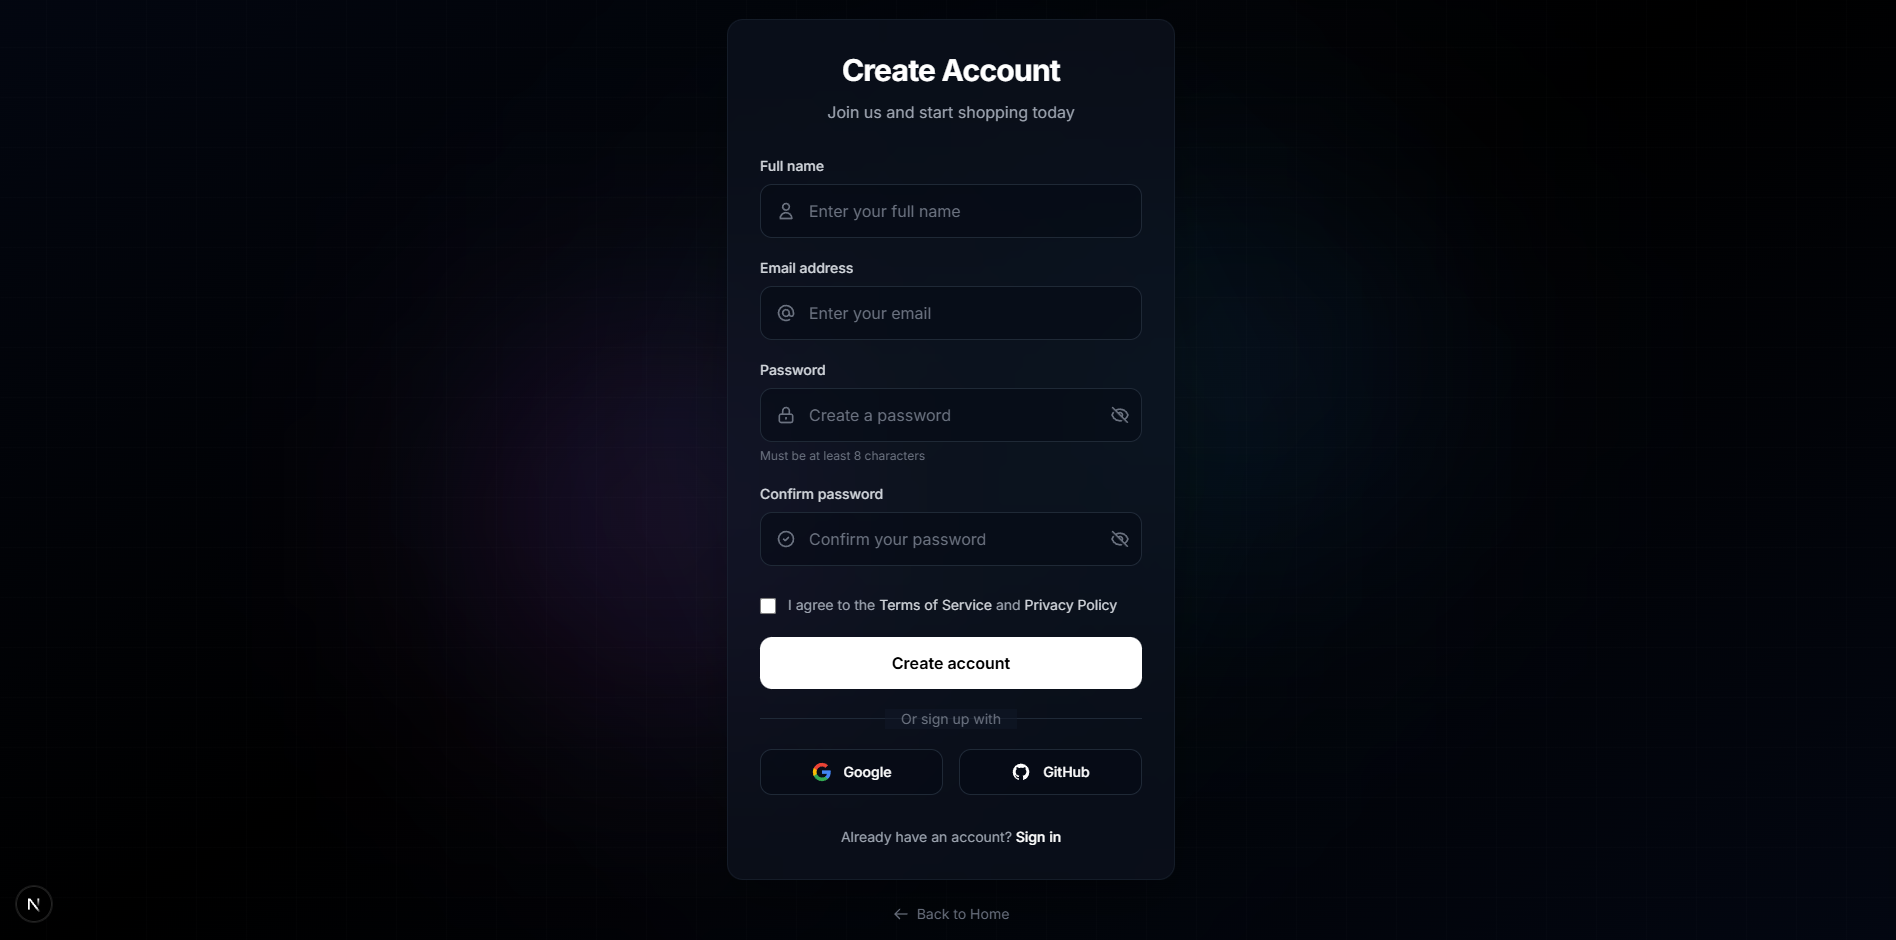
\includegraphics[width=1\textwidth]{image/usecase/dangky.png}
\caption{Giao diện đăng ký vào hệ thống}
\label{fig:mockup-dangky}
\end{figure}

\subsubsection{Giao diện đăng nhập}
Giao diện xác thực người dùng với email và mật khẩu. Tùy chọn "Ghi nhớ đăng nhập".

\begin{figure}[H]
\centering
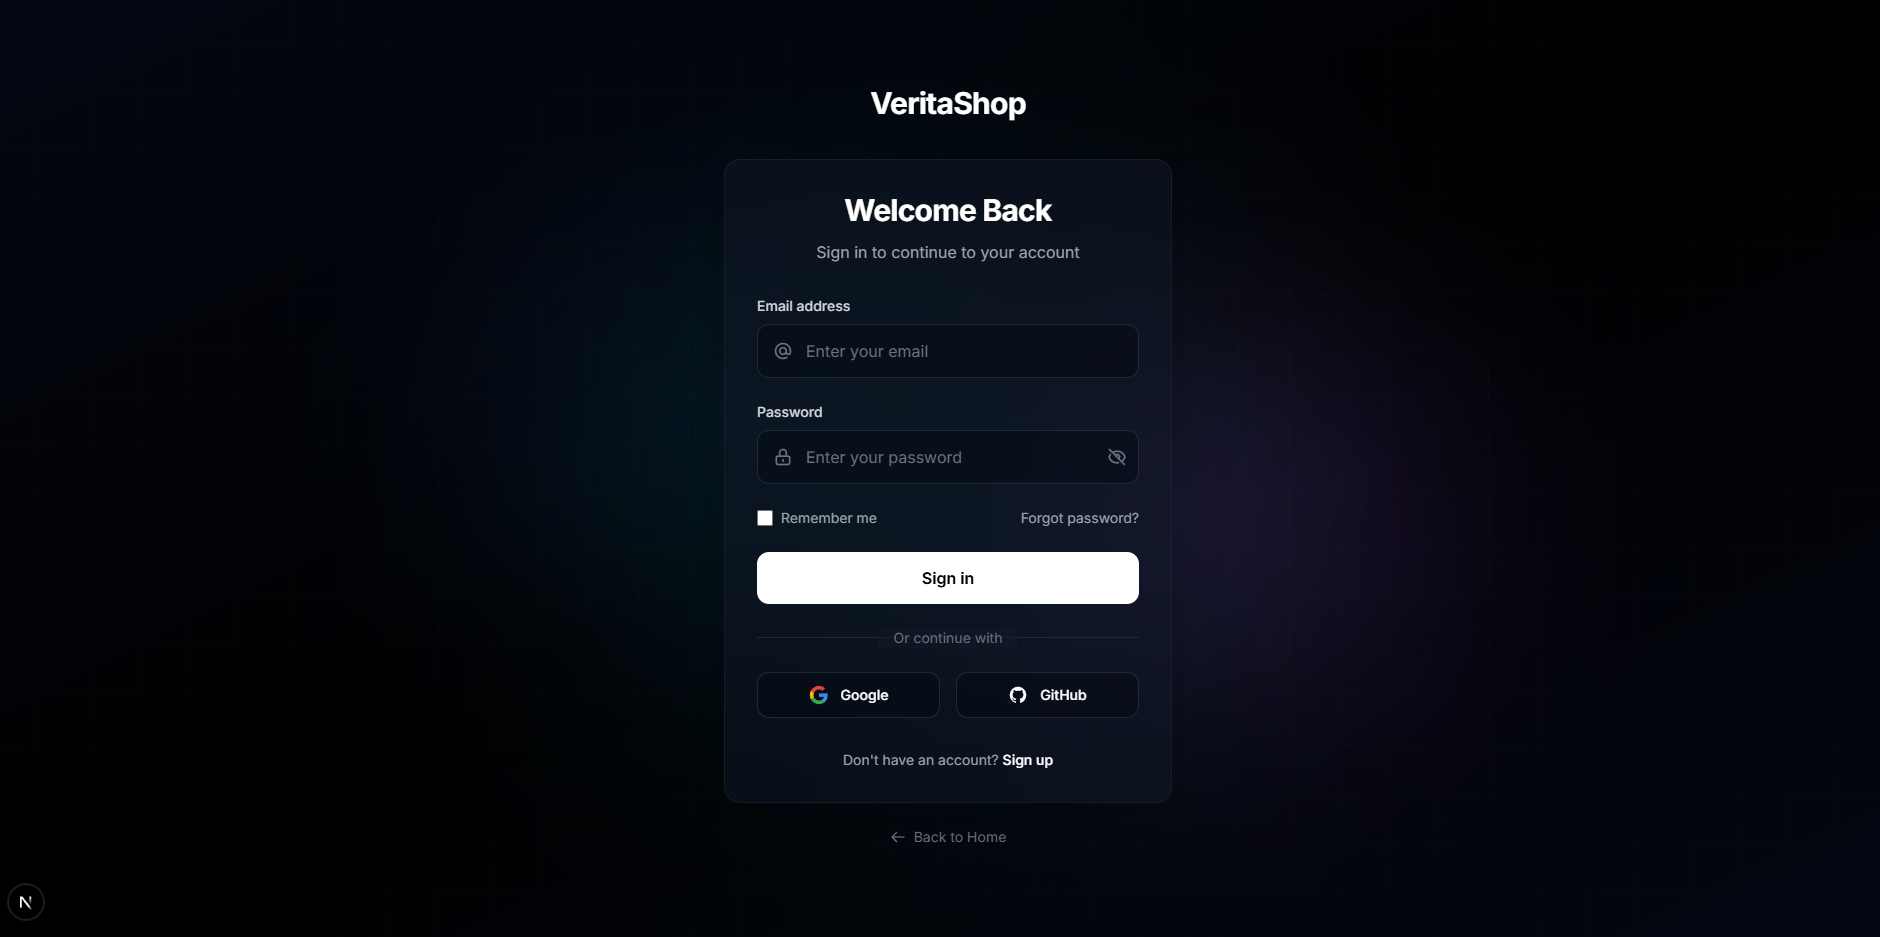
\includegraphics[width=1\textwidth]{image/usecase/dangnhap.png}
\caption{Giao diện đăng nhập vào hệ thống}
\label{fig:mockup-dangnhap}
\end{figure}

\subsubsection{Giao diện hiển thị sản phẩm}
Trang danh sách sản phẩm là giao diện chính để người dùng duyệt và tìm kiếm sản phẩm trên VeritaShop. Dữ liệu được tải từ API \texttt{GET /api/products} (public, không yêu cầu xác thực) với cơ chế phân trang (pagination). Các tham số truy vấn gồm: \texttt{page} (số trang, mặc định \texttt{0}, validation \texttt{@Min(0)}), \texttt{size} (số sản phẩm mỗi trang, mặc định \texttt{20}, validation \texttt{@Min(1) @Max(100)}) và \texttt{categoryId} (tùy chọn -- lọc sản phẩm theo danh mục). API trả về đối tượng \texttt{Page<ProductResponse>} chứa danh sách sản phẩm cùng metadata phân trang: tổng số phần tử, tổng số trang, trang hiện tại và kích thước trang.

Mỗi sản phẩm trong danh sách được hiển thị dưới dạng thẻ (card) trong bố cục lưới (grid), thông tin lấy từ \texttt{ProductResponse} gồm: ảnh đại diện (\texttt{image} -- URL ảnh từ Cloudinary), tên sản phẩm (\texttt{name} -- trường có \texttt{@Indexed} trong MongoDB để tăng tốc tìm kiếm), thương hiệu (\texttt{brand}), giá bán hiện tại (\texttt{price}), giá gốc (\texttt{originalPrice} -- nếu khác giá bán sẽ hiển thị giá gốc bị gạch ngang cùng phần trăm giảm giá), điểm đánh giá trung bình (\texttt{rating} -- số sao từ 0.0 đến 5.0, được tính tự động từ trung bình cộng tất cả review) và badge khuyến mãi (\texttt{badge} -- ví dụ ''Giảm giá'', ''Mới'', hiển thị dưới dạng nhãn nổi góc trên ảnh sản phẩm). Ngoài ra, mỗi card còn hiển thị tên danh mục (\texttt{categoryName}) được resolve từ \texttt{categoryId}.

Phía trên danh sách sản phẩm là thanh bộ lọc cho phép: lọc theo danh mục (dropdown hoặc tabs ngang, gửi tham số \texttt{categoryId} khi gọi API), sắp xếp theo tiêu chí (giá tăng dần, giá giảm dần, mới nhất, đánh giá cao nhất). Bên dưới là thanh phân trang (pagination bar) hiển thị số trang và nút chuyển trang, tương ứng với tham số \texttt{page} và \texttt{size} của API. Trong entity \texttt{Product}, trường \texttt{stock} tổng hợp tồn kho từ tất cả biến thể (variants) -- sản phẩm hết hàng (\texttt{stock = 0}) sẽ hiển thị nhãn ''Hết hàng'' và vô hiệu hóa nút thêm giỏ. Repository sử dụng \texttt{Page<Product> findByCategoryId(String categoryId, Pageable pageable)} để truy vấn có phân trang theo danh mục.

\begin{figure}[H]
\centering
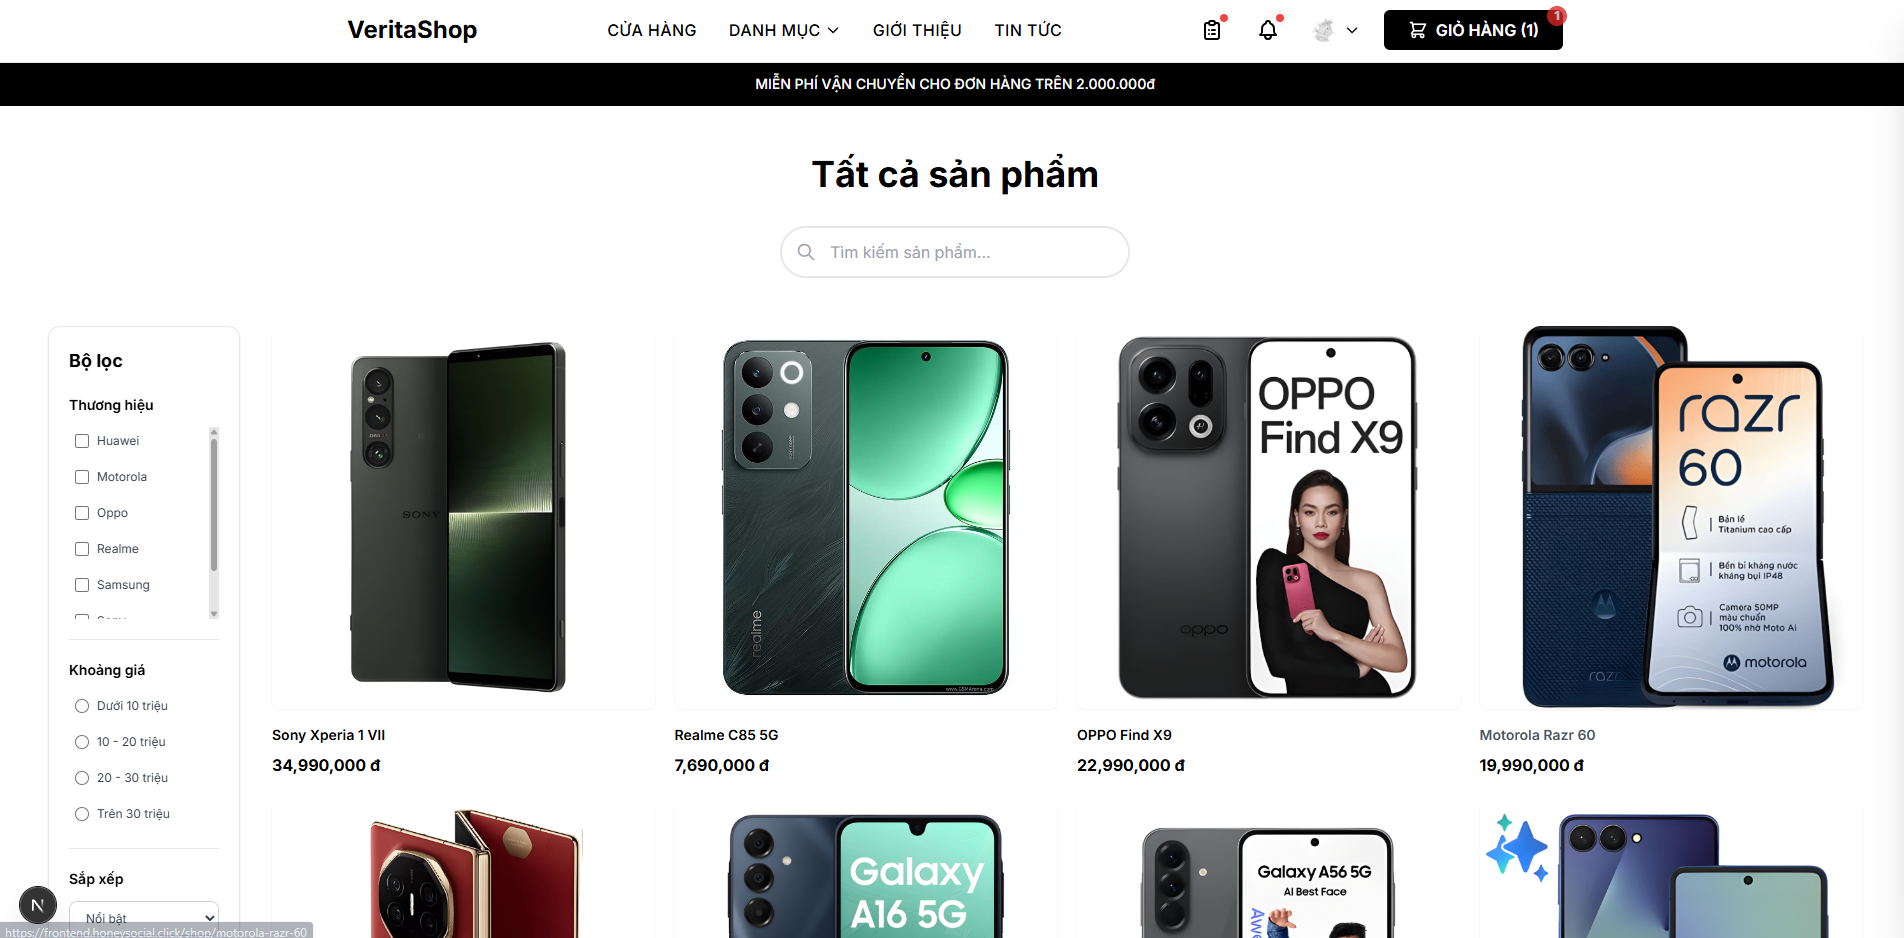
\includegraphics[width=1\textwidth]{image/usecase/hien-thi-sp.png}
\caption{Giao diện hiển thị sản phẩm}
\label{fig:mockup-hienthi-sp}
\end{figure}

\subsubsection{Giao diện chi tiết sản phẩm}
Trang chi tiết sản phẩm hiển thị toàn bộ thông tin của một sản phẩm cụ thể, dữ liệu lấy từ API \texttt{GET /api/products/\{id\}} (public, không yêu cầu xác thực). API trả về đối tượng \texttt{ProductResponse} đầy đủ gồm: \texttt{id} (mã sản phẩm duy nhất trong MongoDB), \texttt{name} (tên sản phẩm), \texttt{brand} (thương hiệu -- ví dụ Apple, Samsung, Xiaomi), \texttt{categoryId} và \texttt{categoryName} (danh mục sản phẩm), \texttt{price} (giá bán hiện tại), \texttt{originalPrice} (giá gốc trước giảm giá, có thể null), \texttt{image} (ảnh đại diện chính từ Cloudinary), \texttt{rating} (điểm đánh giá trung bình 0.0--5.0, được tính tự động từ trung bình cộng tất cả review và làm tròn 1 chữ số thập phân), \texttt{badge} (nhãn khuyến mãi), \texttt{specs} (thông số kỹ thuật dạng chuỗi), \texttt{stock} (tổng số lượng tồn kho từ tất cả biến thể), \texttt{createdAt} và \texttt{updatedAt} (thời gian tạo và cập nhật).

Điểm đặc biệt của trang chi tiết là phần hiển thị biến thể sản phẩm (variants). Mỗi sản phẩm có thể có nhiều biến thể, mỗi biến thể là một đối tượng \texttt{ProductVariant} gồm: \texttt{color} (màu sắc -- ví dụ ''Đen'', ''Trắng'', ''Xanh dương''), \texttt{storage} (dung lượng bộ nhớ -- ví dụ ''128GB'', ''256GB'', ''512GB''), \texttt{image} (ảnh riêng của biến thể, thay đổi khi chọn màu khác), \texttt{price} (giá riêng của biến thể -- có thể khác nhau giữa các dung lượng) và \texttt{stock} (tồn kho riêng của biến thể). Giao diện hiển thị các lựa chọn màu sắc dưới dạng các ô tròn/vuông có màu tương ứng, khi người dùng chọn màu thì ảnh sản phẩm thay đổi sang \texttt{image} của biến thể đó. Các lựa chọn dung lượng hiển thị dưới dạng các nút (button), khi chọn dung lượng thì giá cập nhật theo \texttt{price} của biến thể. Nếu biến thể hết hàng (\texttt{stock = 0}), nút dung lượng đó bị mờ và không cho chọn.

Entity \texttt{Product} sử dụng \texttt{@Version Long version} cho Optimistic Locking, đảm bảo không xảy ra xung đột khi nhiều người cùng mua sản phẩm cuối cùng trong kho. Trong service layer, phương thức \texttt{syncSummaryFieldsFromVariants()} tự động đồng bộ: giá chính của sản phẩm (\texttt{price}) lấy từ biến thể đầu tiên (primary variant) và tổng tồn kho (\texttt{stock}) bằng tổng \texttt{stock} của tất cả biến thể.

Phần dưới trang gồm: nút ''Thêm vào giỏ hàng'' (gọi \texttt{POST /api/cart/items} với \texttt{CartItemRequest} chứa \texttt{productId}, \texttt{color}, \texttt{storage} đã chọn và \texttt{quantity}), nút ''Mua ngay'' (thêm vào giỏ rồi chuyển thẳng sang trang thanh toán) và nút yêu thích (biểu tượng trái tim, gọi \texttt{POST /api/wishlist/\{productId\}} để toggle). Phần thông số kỹ thuật (\texttt{specs}) hiển thị dưới dạng bảng hoặc danh sách key-value. Khu vực bình luận và đánh giá sản phẩm nằm phía dưới cùng.

\begin{figure}[H]
\centering
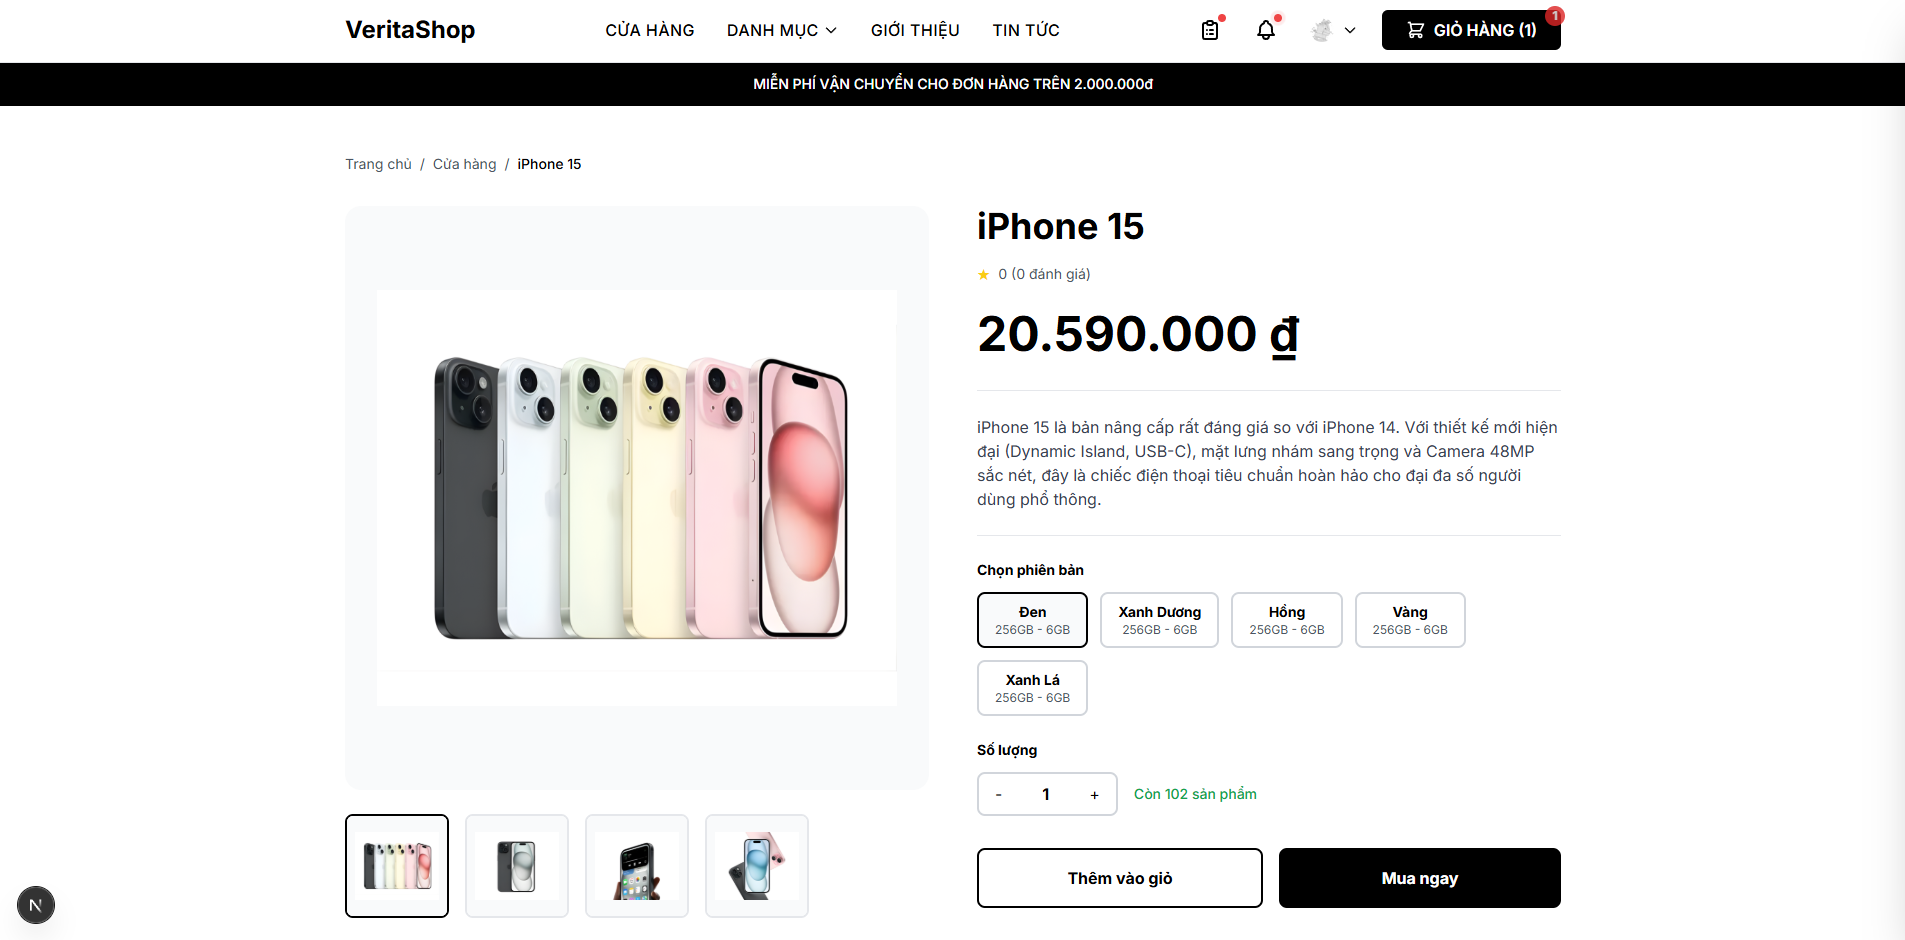
\includegraphics[width=1\textwidth]{image/usecase/chi-tiet-sp.png}
\caption{Giao diện chi tiết sản phẩm}
\label{fig:mockup-chitiet-sp}
\end{figure}

\subsubsection{Giao diện bình luận sản phẩm}
Khu vực bình luận (review) nằm trong trang chi tiết sản phẩm, hiển thị tất cả đánh giá của người dùng đã mua sản phẩm cùng kết quả phân tích cảm xúc tự động bằng AI. Danh sách bình luận được tải từ API \texttt{GET /api/reviews?productId=\{productId\}} (public, không yêu cầu xác thực), trả về \texttt{List<ReviewResponse>} sắp xếp theo \texttt{createdAt} mới nhất lên đầu (query \texttt{findByProductIdOrderByCreatedAtDesc} trong repository).

Mỗi bình luận (\texttt{ReviewResponse}) hiển thị đầy đủ: tên người dùng (\texttt{username}), số sao đánh giá (\texttt{rating} -- từ 1 đến 5, hiển thị bằng biểu tượng sao vàng), nội dung bình luận (\texttt{comment}), danh sách ảnh đính kèm (\texttt{images} -- tối đa 5 ảnh, hiển thị dạng gallery thu nhỏ có thể click phóng to), thời gian đăng (\texttt{createdAt}) và quan trọng nhất là kết quả phân tích cảm xúc (\texttt{analysisResults}).

Kết quả phân tích cảm xúc \texttt{analysisResults} là một danh sách \texttt{List<ReviewAspectAnalysis>}, mỗi phần tử chứa ba trường: \texttt{aspect} (khía cạnh được đề cập trong bình luận -- ví dụ ''chất lượng'', ''pin'', ''camera'', ''màn hình'', ''giá cả'', ''vận chuyển''), \texttt{sentiment} (cảm xúc của người dùng về khía cạnh đó -- POSITIVE, NEGATIVE hoặc NEUTRAL) và \texttt{confidence} (độ tin cậy của dự đoán, giá trị từ 0.0 đến 1.0). Giao diện hiển thị mỗi khía cạnh dưới dạng badge màu: xanh lá cho POSITIVE, đỏ cho NEGATIVE và xám cho NEUTRAL, kèm theo tên khía cạnh và phần trăm độ tin cậy.

Cơ chế phân tích cảm xúc hoạt động như sau: khi người dùng gửi bình luận mới qua API \texttt{POST /api/reviews} (yêu cầu \texttt{@PreAuthorize("hasRole('USER')")}), backend gọi \texttt{AbsaService.analyzeComment(comment)} để phân tích. Cụ thể, \texttt{AbsaServiceImpl} gửi HTTP POST đến microservice Python tại \texttt{\$\{absa.api-url\}/predict} (mặc định \texttt{http://localhost:9000/predict}) với body \texttt{AbsaPredictRequest} chứa trường \texttt{text} là nội dung bình luận. Microservice trả về \texttt{AbsaPredictResponse} chứa \texttt{List<ReviewAspectAnalysis> results}. Nếu microservice không khả dụng hoặc trả lỗi, hệ thống vẫn lưu bình luận bình thường nhưng \texttt{analysisResults} sẽ là danh sách rỗng (graceful degradation -- bình luận không bị mất khi AI service down).

Form viết bình luận gồm: dropdown hoặc row sao chọn số sao đánh giá (\texttt{rating}, validation \texttt{@NotNull @Min(1) @Max(5)} -- bắt buộc chọn từ 1 đến 5 sao), ô nhập nội dung bình luận (\texttt{comment}, validation \texttt{@NotBlank @Size(max = 1000)} -- bắt buộc, tối đa 1000 ký tự) và khu vực tải ảnh (\texttt{images}, validation \texttt{@Size(max = 5)} -- tùy chọn, tối đa 5 ảnh). Ảnh được upload trước qua API riêng \texttt{POST /api/reviews/upload-image} (nhận \texttt{MultipartFile}, trả về URL Cloudinary), sau đó URL được gửi kèm trong \texttt{CreateReviewRequest}. Body request đầy đủ gồm: \texttt{productId} (\texttt{@NotBlank}), \texttt{rating}, \texttt{comment} và \texttt{images}.

Hệ thống áp dụng ràng buộc mỗi người dùng chỉ được đánh giá một sản phẩm duy nhất một lần, được đảm bảo bởi \texttt{@CompoundIndex(def = "\{'userId': 1, 'productId': 1\}", unique = true)} trên entity \texttt{Review} trong MongoDB. Nếu người dùng đã đánh giá rồi, hệ thống ném \texttt{DuplicateResourceException}. Tuy nhiên, người dùng có thể chỉnh sửa bình luận đã viết qua API \texttt{PUT /api/reviews/\{id\}} (chỉ chủ sở hữu mới được sửa, validation ownership trong service) -- khi cập nhật, hệ thống gọi lại ABSA service để phân tích lại cảm xúc với nội dung mới. Người dùng cũng có thể xóa bình luận qua \texttt{DELETE /api/reviews/\{id\}} (chỉ chủ sở hữu).

Sau mỗi thao tác tạo, sửa hoặc xóa bình luận, service tự động gọi \texttt{recalculateProductRating()} để tính lại điểm đánh giá trung bình của sản phẩm: lấy trung bình cộng \texttt{rating} của tất cả review, làm tròn 1 chữ số thập phân và cập nhật vào trường \texttt{rating} của entity \texttt{Product}. Điểm này được phản ánh ngay trên trang danh sách sản phẩm và trang chi tiết.

\begin{figure}[H]
\centering
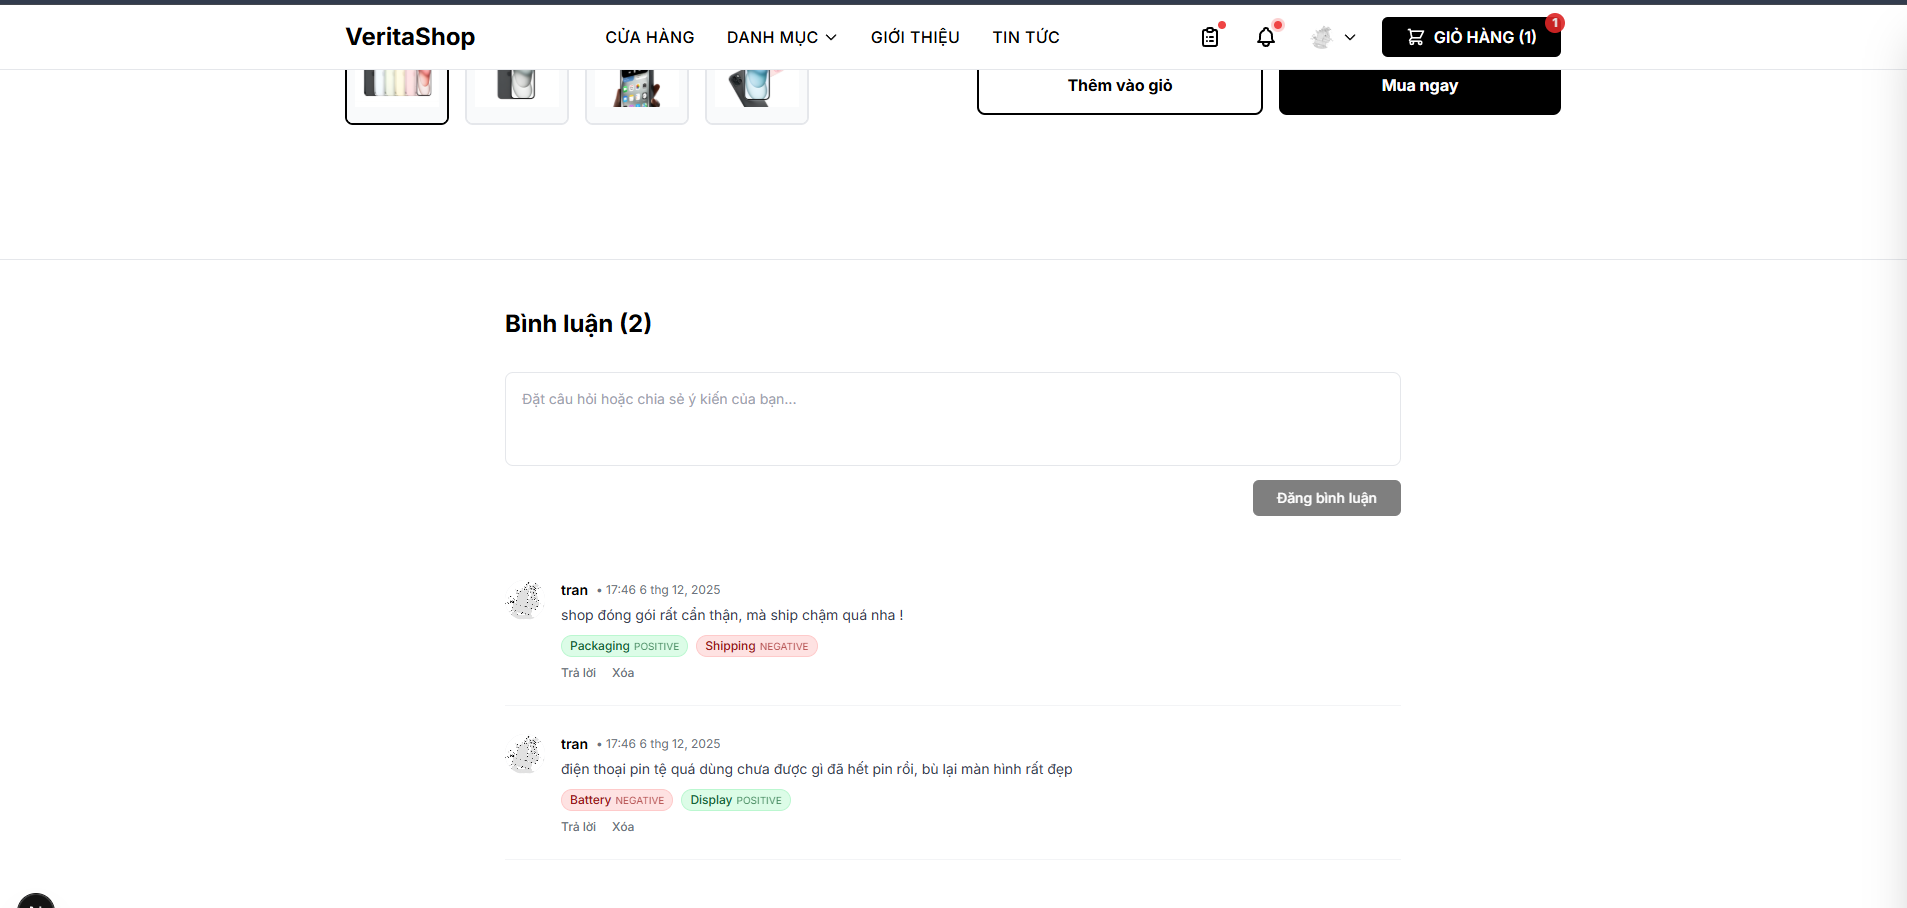
\includegraphics[width=1\textwidth]{image/usecase/binh-luan.png}
\caption{Giao diện bình luận sản phẩm}
\label{fig:mockup-binhluan}
\end{figure}

\subsubsection{Trang tổng quan quản trị (Dashboard)}
Trang tổng quan quản trị (Dashboard) là giao diện đầu tiên mà người quản trị viên (role ADMIN) nhìn thấy khi đăng nhập vào hệ thống VeritaShop. Toàn bộ khu vực quản trị được bảo vệ bởi \texttt{@PreAuthorize("hasRole('ADMIN')")} trên các API endpoint, chỉ cho phép tài khoản có vai trò ADMIN truy cập. Giao diện được bố trí theo hai cột: thanh điều hướng bên trái (sidebar) với nền tối chứa logo VeritaShop và các mục chức năng quản trị -- Tổng quan, Sản phẩm, Thể loại, Đơn hàng, Người dùng, Voucher, Tin nhắn -- mỗi mục đi kèm biểu tượng (icon) tương ứng.

Vùng nội dung chính bên phải hiển thị các thẻ thống kê tổng hợp từ dữ liệu MongoDB: tổng doanh thu (tính từ trường \texttt{total} của các đơn hàng có \texttt{status = DELIVERED}), tổng số đơn hàng, số sản phẩm đang kinh doanh và số người dùng đã đăng ký. Phía dưới là biểu đồ doanh thu theo thời gian giúp theo dõi xu hướng kinh doanh, kèm theo bảng đơn hàng gần đây hiển thị các cột: mã đơn (\texttt{orderCode}), tên khách hàng (\texttt{customerName}), tổng tiền (\texttt{total}), trạng thái đơn hàng và ngày tạo.

\begin{figure}[H]
\centering
\includegraphics[width=1\textwidth]{image/Img/Tong-quan-admin.png}
\caption{Giao diện tổng quan quản trị (Dashboard)}
\label{fig:mockup-dashboard}
\end{figure}

\subsubsection{Trang quản lý sản phẩm}
Trang quản lý sản phẩm gọi API \texttt{GET /api/products?page=\&size=\&categoryId=} để lấy danh sách sản phẩm phân trang từ collection \texttt{products} trên MongoDB. Bảng hiển thị các cột tương ứng với trường dữ liệu trong model \texttt{Product}: hình ảnh đại diện (\texttt{image}), tên sản phẩm (\texttt{name}), thương hiệu (\texttt{brand}), tên danh mục (\texttt{categoryName} -- được resolve từ \texttt{categoryId}), giá bán (\texttt{price}), giá gốc (\texttt{originalPrice}), tồn kho (\texttt{stock}), đánh giá trung bình (\texttt{rating}), badge khuyến mãi (\texttt{badge}), và các nút hành động sửa/xóa.

Thanh công cụ phía trên bảng có ô tìm kiếm lọc theo tên sản phẩm, dropdown lọc theo \texttt{categoryId}, nút ''Thêm sản phẩm'' gọi \texttt{POST /api/products} và nút ''Import Excel'' gọi \texttt{POST /api/products/import/excel}. Hệ thống sử dụng Optimistic Locking (trường \texttt{@Version}) trên Product để tránh xung đột khi nhiều admin cùng chỉnh sửa. Phân trang mặc định 20 sản phẩm/trang (\texttt{size=20}), tối đa 100. Nút xóa gọi \texttt{DELETE /api/products/\{id\}} với xác nhận trước khi thực hiện.

\begin{figure}[H]
\centering
\includegraphics[width=1\textwidth]{image/Img/San-pham-admin.png}
\caption{Giao diện quản lý sản phẩm}
\label{fig:mockup-sanpham-admin}
\end{figure}

\subsubsection{Trang thêm sản phẩm mới}
Form thêm sản phẩm gọi \texttt{POST /api/products} với body theo \texttt{CreateProductRequest}. Các trường bắt buộc (đánh dấu \texttt{@NotBlank}): tên sản phẩm (\texttt{name}), thương hiệu (\texttt{brand}), URL hình ảnh (\texttt{image}). Các trường tùy chọn: danh mục (\texttt{categoryId} -- dropdown chọn từ danh sách category), giá bán (\texttt{price}, \texttt{@Min(0)}), giá gốc (\texttt{originalPrice}), đánh giá (\texttt{rating}, mặc định 0.0), badge (\texttt{badge}), thông số kỹ thuật (\texttt{specs}), tồn kho (\texttt{stock}, \texttt{@Min(0)}, mặc định 0).

Phần quan trọng nhất là danh sách biến thể (\texttt{variants}) -- mỗi \texttt{ProductVariant} gồm: màu sắc (\texttt{color}), dung lượng bộ nhớ (\texttt{storage}), URL hình ảnh riêng (\texttt{image}), giá riêng (\texttt{price}) và tồn kho riêng (\texttt{stock}). Đây là tính năng đặc trưng cho sản phẩm điện thoại vì mỗi model có nhiều phiên bản màu/bộ nhớ khác nhau. Form cho phép thêm/xóa động từng variant. Hình ảnh sản phẩm được upload lên Cloudinary thông qua \texttt{POST /api/upload} và lưu URL trả về.

\begin{figure}[H]
\centering
\includegraphics[width=1\textwidth]{image/Img/Them-san-pham.png}
\caption{Giao diện thêm sản phẩm mới}
\label{fig:mockup-themsanpham}
\end{figure}

\subsubsection{Trang import sản phẩm từ Excel}
Tính năng import hàng loạt gọi \texttt{POST /api/products/import/excel} (\texttt{consumes = MULTIPART\_FORM\_DATA}) với file \texttt{.xlsx} hoặc \texttt{.xls}. Server tạo một \texttt{ProductImportJob} trong collection \texttt{product\_import\_jobs} với trạng thái ban đầu \texttt{QUEUED}, sau đó xử lý bất đồng bộ qua \texttt{@Async("productImportExecutor")}. Frontend theo dõi tiến trình bằng cách polling \texttt{GET /api/products/import/\{jobId\}}.

Giao diện gồm hai phần: vùng upload file (kéo thả hoặc chọn file) và bảng theo dõi tiến trình. Bảng hiển thị các trường từ \texttt{ProductImportJobResponse}: tên file gốc (\texttt{originalFileName}), trạng thái (\texttt{status} -- QUEUED, PROCESSING, COMPLETED, COMPLETED\_WITH\_ERRORS, FAILED), tổng số dòng (\texttt{totalRows}), số dòng đã xử lý (\texttt{processedRows}), thành công (\texttt{successCount}), thất bại (\texttt{failureCount}), thời gian bắt đầu/hoàn thành, thông báo tóm tắt (\texttt{summaryMessage}) và danh sách lỗi chi tiết (\texttt{errors}) gồm số dòng (\texttt{rowNumber}) và nội dung lỗi (\texttt{message}), giới hạn tối đa 200 lỗi.

\begin{figure}[H]
\centering
\includegraphics[width=1\textwidth]{image/Img/import-excel-san-pham.png}
\caption{Giao diện import sản phẩm từ Excel}
\label{fig:mockup-import-excel}
\end{figure}

\subsubsection{Trang quản lý thể loại (danh mục)}
Trang quản lý thể loại gọi \texttt{GET /api/categories} để lấy toàn bộ danh mục từ collection \texttt{categories}. Bảng hiển thị các cột theo \texttt{CategoryResponse}: tên danh mục (\texttt{name}), slug URL (\texttt{slug}), mô tả (\texttt{description}), icon (\texttt{icon}), số lượng sản phẩm thuộc danh mục (\texttt{productCount}) và ngày tạo (\texttt{createdAt}). Mỗi danh mục có ràng buộc \texttt{@Indexed(unique = true)} trên trường \texttt{name}, đảm bảo không trùng tên.

Thanh công cụ phía trên bảng có nút ''Thêm danh mục'' và ô tìm kiếm. Cột hành động gồm nút sửa (gọi \texttt{PUT /api/categories/\{id\}}) và nút xóa (gọi \texttt{DELETE /api/categories/\{id\}?force=false}). Khi \texttt{force=false}, hệ thống từ chối xóa danh mục đang có sản phẩm; khi \texttt{force=true} sẽ xóa kể cả khi có sản phẩm liên quan. Hộp thoại xác nhận hiện lên trước khi xóa, cảnh báo nếu danh mục đang chứa sản phẩm.

\begin{figure}[H]
\centering
\includegraphics[width=1\textwidth]{image/Img/The-loai-admin.png}
\caption{Giao diện quản lý thể loại sản phẩm}
\label{fig:mockup-theloai-admin}
\end{figure}

\subsubsection{Trang thêm danh mục mới}
Form thêm danh mục gọi \texttt{POST /api/categories} với body theo \texttt{CreateCategoryRequest}. Trường bắt buộc: tên danh mục (\texttt{name}, \texttt{@NotBlank} với message ''Category name is required''). Các trường tùy chọn: mô tả (\texttt{description}) và icon (\texttt{icon}). Hệ thống tự động tạo \texttt{slug} từ tên danh mục phía backend (chuyển sang chữ thường, bỏ dấu tiếng Việt, thay khoảng trắng bằng dấu gạch ngang).

Form được bố trí trên một card nền trắng, gồm ba trường nhập liệu xếp dọc. Trường tên danh mục hiển thị dấu (*) bắt buộc, với thông báo lỗi validation ngay bên dưới nếu để trống. Trường icon cho phép nhập URL icon hoặc tên icon class. Hai nút hành động ở cuối form: ''Lưu'' (submit) và ''Hủy'' (quay lại trang danh sách).

\begin{figure}[H]
\centering
\includegraphics[width=1\textwidth]{image/Img/Them-danh-muc.png}
\caption{Giao diện thêm danh mục mới}
\label{fig:mockup-themdanhmuc}
\end{figure}

\subsubsection{Trang quản lý đơn hàng}
Trang quản lý đơn hàng gọi \texttt{GET /api/orders?page=\&size=} để lấy danh sách phân trang từ collection \texttt{orders}. Bảng hiển thị các cột theo \texttt{OrderResponse}: mã đơn hàng (\texttt{orderCode} -- mã duy nhất với \texttt{@Indexed(unique = true)} ngăn đơn trùng lặp nhờ idempotency key), tên khách hàng (\texttt{customerName}), email (\texttt{email}), số điện thoại (\texttt{phone}), tổng tiền (\texttt{total}), phương thức thanh toán (\texttt{paymentMethod} -- COD hoặc MoMo), trạng thái thanh toán (\texttt{paymentStatus} -- PENDING/PAID/FAILED), trạng thái đơn hàng (\texttt{status}) và ngày tạo.

Cột trạng thái đơn hàng sử dụng badge màu tương ứng với 5 giá trị enum \texttt{OrderStatus}: PENDING (vàng), CONFIRMED (xanh dương), SHIPPING (cam), DELIVERED (xanh lá), CANCELLED (đỏ). Admin cập nhật trạng thái qua \texttt{PATCH /api/orders/\{id\}/status?status=...}. Đơn hàng có thể bị hủy qua \texttt{PATCH /api/orders/\{id\}/cancel?reason=...}, khi đó lưu \texttt{cancelReason} và \texttt{cancelledBy} (USER hoặc ADMIN). Đơn thanh toán MoMo hiển thị thêm \texttt{momoTransId}. Thông tin giao hàng gồm: địa chỉ (\texttt{address}), quận/huyện (\texttt{district}), phường/xã (\texttt{ward}), thành phố (\texttt{city}). Bảng mặc định 20 dòng/trang.

\begin{figure}[H]
\centering
\includegraphics[width=1\textwidth]{image/Img/Don-hang-admin.png}
\caption{Giao diện quản lý đơn hàng}
\label{fig:mockup-donhang-admin}
\end{figure}

\subsubsection{Trang quản lý người dùng}
Trang quản lý người dùng gọi \texttt{GET /api/users?page=\&size=} để lấy danh sách phân trang (mặc định 10 người/trang, tối đa 100) từ collection \texttt{users}. Bảng hiển thị các cột theo \texttt{UserResponse}: tên đăng nhập (\texttt{username}), email (\texttt{email}), vai trò (\texttt{role} -- chỉ có 2 giá trị: USER và ADMIN theo enum \texttt{Role}), trạng thái khóa (\texttt{banned} -- true/false), phương thức xác thực (\texttt{authProvider} -- LOCAL cho đăng ký thường, GOOGLE cho đăng nhập Google, GOOGLE\_AND\_LOCAL cho cả hai), trạng thái mật khẩu (\texttt{hasPassword}) và ngày tạo (\texttt{createdAt}).

Cột hành động cung cấp hai chức năng quản trị: thay đổi vai trò qua \texttt{PATCH /api/users/\{id\}/role?role=...} và khóa/mở khóa tài khoản qua \texttt{PATCH /api/users/\{id\}/ban}. Hệ thống có bảo vệ: admin không thể tự khóa hoặc đổi vai trò của chính mình (kiểm tra \texttt{requesterId.equals(id)} sẽ throw \texttt{BadRequestException}). Cột vai trò hiển thị badge với mã màu phân biệt USER và ADMIN. Cột trạng thái khóa hiển thị biểu tượng khóa/mở khóa trực quan.

\begin{figure}[H]
\centering
\includegraphics[width=1\textwidth]{image/Img/Nguoi-dung-admin.png}
\caption{Giao diện quản lý người dùng}
\label{fig:mockup-nguoidung-admin}
\end{figure}

\subsubsection{Trang quản lý Voucher (mã giảm giá)}
Trang quản lý voucher gọi \texttt{GET /api/vouchers} để lấy toàn bộ mã giảm giá từ collection \texttt{vouchers}. Bảng hiển thị các cột theo \texttt{VoucherResponse}: mã voucher (\texttt{code} -- \texttt{@Indexed(unique = true)}), mô tả (\texttt{description}), loại voucher (\texttt{type} -- PRODUCT cho giảm giá sản phẩm, SHIPPING cho giảm phí vận chuyển), kiểu giảm (\texttt{discountType} -- PERCENTAGE cho phần trăm, FIXED\_AMOUNT cho số tiền cố định), giá trị giảm (\texttt{discountValue}), giảm tối đa (\texttt{maxDiscountAmount}), đơn tối thiểu (\texttt{minOrderValue}), số lần đã dùng/tổng số lần (\texttt{usedCount}/\texttt{usageLimit}), ngày bắt đầu (\texttt{startAt}), ngày kết thúc (\texttt{endAt}) và trạng thái (\texttt{active}).

Thanh công cụ có nút ''Tạo voucher'' và ô tìm kiếm. Cột hành động gồm nút sửa (gọi \texttt{PUT /api/vouchers/\{id\}}) và nút xóa (gọi \texttt{DELETE /api/vouchers/\{id\}}). Cột trạng thái hiển thị badge: xanh lá cho active=true, đỏ cho active=false hoặc đã quá ngày \texttt{endAt}. Bảng phân biệt rõ voucher sản phẩm (PRODUCT) và voucher vận chuyển (SHIPPING) bằng badge loại khác nhau.

\begin{figure}[H]
\centering
\includegraphics[width=1\textwidth]{image/Img/Voucher-admin.png}
\caption{Giao diện quản lý Voucher}
\label{fig:mockup-voucher-admin}
\end{figure}

\subsubsection{Trang tạo Voucher mới}
Form tạo voucher gọi \texttt{POST /api/vouchers} với body theo \texttt{CreateVoucherRequest}. Trường bắt buộc: mã voucher (\texttt{code}, \texttt{@NotBlank}), loại voucher (\texttt{type}, \texttt{@NotNull} -- dropdown chọn PRODUCT hoặc SHIPPING), kiểu giảm giá (\texttt{discountType}, \texttt{@NotNull} -- dropdown chọn PERCENTAGE hoặc FIXED\_AMOUNT). Trường có validation số: giá trị giảm (\texttt{discountValue}, \texttt{@DecimalMin("0.0")}), giảm tối đa (\texttt{maxDiscountAmount}, \texttt{@DecimalMin("0.0")}), đơn hàng tối thiểu (\texttt{minOrderValue}, \texttt{@DecimalMin("0.0")}). Các trường khác: mô tả (\texttt{description}), giới hạn số lần sử dụng (\texttt{usageLimit}), ngày bắt đầu (\texttt{startAt}), ngày kết thúc (\texttt{endAt}) và trạng thái kích hoạt (\texttt{active}).

Form được chia thành các nhóm logic: thông tin cơ bản (mã, mô tả), loại và điều kiện áp dụng (type, discountType, discountValue, maxDiscountAmount, minOrderValue), giới hạn (usageLimit) và thời gian hiệu lực (startAt, endAt). Trường ngày tháng sử dụng date-time picker. Checkbox ''Kích hoạt'' cho phép bật/tắt voucher ngay khi tạo.

\begin{figure}[H]
\centering
\includegraphics[width=1\textwidth]{image/Img/Tao-voucher.png}
\caption{Giao diện tạo Voucher mới}
\label{fig:mockup-tao-voucher}
\end{figure}

\subsubsection{Trang tin nhắn (Chat hỗ trợ khách hàng)}
Trang chat dành cho admin gọi \texttt{GET /api/chat/admin/conversations} để lấy danh sách hội thoại từ collection \texttt{chat\_conversations}, sắp xếp theo \texttt{updatedAt} mới nhất. Giao diện chia làm hai cột. Cột trái hiển thị danh sách hội thoại, mỗi hội thoại gồm: tên người dùng (\texttt{username}), email (\texttt{userEmail}), preview tin nhắn cuối (\texttt{lastMessagePreview} -- hiển thị ''[Hình ảnh]'' nếu tin nhắn cuối là IMAGE), tên người gửi cuối (\texttt{lastMessageSenderName}) và badge đếm tin chưa đọc (\texttt{unreadCountForAdmin}).

Khi chọn một hội thoại, cột phải gọi \texttt{GET /api/chat/admin/conversations/\{conversationId\}/messages} để load lịch sử tin nhắn từ collection \texttt{chat\_messages}. Mỗi tin nhắn (\texttt{ChatMessageResponse}) hiển thị: nội dung (\texttt{content}), tên người gửi (\texttt{senderName}), vai trò (\texttt{senderRole} -- USER hoặc ADMIN), loại tin nhắn (\texttt{type} -- TEXT hiển thị văn bản, IMAGE hiển thị hình ảnh inline), trạng thái đã đọc (\texttt{readByUser}/\texttt{readByAdmin}) và thời gian gửi (\texttt{createdAt}). Admin gửi tin nhắn qua \texttt{POST /api/chat/admin/messages} với body gồm \texttt{conversationId}, \texttt{content} và \texttt{type}. Hệ thống sử dụng WebSocket (STOMP/SockJS) để broadcast tin nhắn realtime qua các topic: \texttt{/topic/admin/chat/conversations} (cập nhật danh sách hội thoại), \texttt{/topic/admin/chat/messages} (tin nhắn mới) và \texttt{/user/\{userId\}/queue/chat/messages} (gửi riêng cho user).

\begin{figure}[H]
\centering
\includegraphics[width=1\textwidth]{image/Img/Tin-nhan-admin.png}
\caption{Giao diện tin nhắn hỗ trợ khách hàng}
\label{fig:mockup-tinnhan-admin}
\end{figure}

\subsubsection{Trang giỏ hàng}
Trang giỏ hàng hiển thị toàn bộ sản phẩm mà người dùng đã thêm vào giỏ, dữ liệu được lấy từ API \texttt{GET /api/cart} (yêu cầu xác thực \texttt{@PreAuthorize("hasRole('USER')")}). Hệ thống trả về đối tượng \texttt{CartResponse} gồm các trường: \texttt{id} (mã giỏ hàng), \texttt{userId} (mã người dùng sở hữu giỏ), danh sách \texttt{items} và \texttt{updatedAt} (thời điểm cập nhật cuối cùng). Mỗi phần tử trong danh sách \texttt{items} là một \texttt{CartItem} chứa đầy đủ thông tin sản phẩm: \texttt{productId} (mã sản phẩm), \texttt{productName} (tên sản phẩm), \texttt{productImage} (đường dẫn ảnh đại diện), \texttt{brand} (thương hiệu), \texttt{color} (màu sắc biến thể đã chọn), \texttt{storage} (dung lượng bộ nhớ đã chọn), \texttt{price} (đơn giá tại thời điểm thêm giỏ) và \texttt{quantity} (số lượng).

Giao diện hiển thị mỗi sản phẩm trên một dòng với ảnh thu nhỏ bên trái, bên phải là tên sản phẩm cùng thông tin biến thể (màu sắc, dung lượng), đơn giá và bộ điều khiển tăng/giảm số lượng. Khi người dùng thay đổi số lượng, frontend gọi \texttt{PUT /api/cart/items/\{productId\}?color=\&storage=\&quantity=} để cập nhật, trong đó \texttt{quantity} phải nằm trong khoảng \texttt{@Min(1)} đến \texttt{@Max(99)} theo validation của \texttt{CartItemRequest}. Nút xóa sản phẩm gọi \texttt{DELETE /api/cart/items/\{productId\}?color=\&storage=} để loại bỏ đúng biến thể khỏi giỏ. Phía dưới danh sách có dòng tổng tiền tạm tính và nút ''Tiến hành thanh toán'' dẫn sang trang checkout.

Đặc biệt, hệ thống hỗ trợ đồng bộ giỏ hàng giữa trạng thái khách (guest) và tài khoản đã đăng nhập thông qua API \texttt{POST /api/cart/sync} với body \texttt{CartSyncRequest} chứa \texttt{List<CartItemRequest> items}. Khi người dùng đăng nhập, các sản phẩm đã thêm vào localStorage lúc chưa đăng nhập sẽ được merge với giỏ hàng trên server -- nếu cùng sản phẩm cùng biến thể thì lấy số lượng lớn hơn (higher quantity wins), tổng số lượng mỗi sản phẩm không vượt quá 99. Ngoài ra, API \texttt{DELETE /api/cart} cho phép xóa toàn bộ giỏ hàng khi cần.

\begin{figure}[H]
\centering
\includegraphics[width=1\textwidth]{image/Img/Gio-hang.png}
\caption{Giao diện giỏ hàng}
\label{fig:mockup-gio-hang}
\end{figure}

\subsubsection{Trang thanh toán}
Trang thanh toán là bước cuối cùng trước khi đơn hàng được tạo, giao diện thu thập toàn bộ thông tin giao hàng và phương thức thanh toán. Khi người dùng nhấn ''Đặt hàng'', frontend gọi \texttt{POST /api/orders} (yêu cầu \texttt{@PreAuthorize("hasRole('USER')")}) với body theo cấu trúc \texttt{CreateOrderRequest}. Các trường thông tin giao hàng bắt buộc gồm: \texttt{email} (\texttt{@NotBlank @Email} -- email nhận thông báo), \texttt{customerName} (\texttt{@NotBlank} -- họ tên người nhận), \texttt{phone} (\texttt{@NotBlank} -- số điện thoại liên hệ), \texttt{address} (\texttt{@NotBlank} -- địa chỉ chi tiết: số nhà, tên đường), \texttt{city} (\texttt{@NotBlank} -- tỉnh/thành phố), \texttt{district} (\texttt{@NotBlank} -- quận/huyện) và \texttt{ward} (\texttt{@NotBlank} -- phường/xã). Trường tùy chọn \texttt{note} cho phép người mua ghi chú thêm cho đơn hàng.

Phần chọn phương thức thanh toán sử dụng trường \texttt{paymentMethod} với hai giá trị: COD (thanh toán khi nhận hàng) và MOMO (thanh toán qua ví điện tử MoMo). Nếu chọn MOMO, sau khi tạo đơn hàng thành công, hệ thống sẽ tự động chuyển hướng người dùng sang cổng thanh toán MoMo để hoàn tất giao dịch.

Phần áp dụng mã giảm giá có hai ô nhập: \texttt{productVoucherCode} (mã voucher giảm giá sản phẩm, loại PRODUCT) và \texttt{shippingVoucherCode} (mã voucher miễn phí vận chuyển, loại SHIPPING). Hệ thống cho phép áp dụng đồng thời cả hai loại voucher trên cùng một đơn hàng.

Danh sách sản phẩm đặt mua nằm trong trường \texttt{items} (\texttt{@NotEmpty}), mỗi phần tử là một \texttt{OrderItemRequest} gồm: \texttt{productId} (\texttt{@NotBlank}), \texttt{color} (màu sắc), \texttt{storage} (dung lượng), \texttt{quantity} (\texttt{@Min(1)}) và \texttt{price} (\texttt{@DecimalMin("0.0")}). Trường \texttt{idempotencyKey} (\texttt{@NotBlank}) đảm bảo không tạo đơn hàng trùng lặp khi người dùng nhấn nút ''Đặt hàng'' nhiều lần -- frontend tạo UUID duy nhất cho mỗi lần checkout.

Giao diện chia thành hai cột: cột trái chứa form nhập thông tin giao hàng và phương thức thanh toán, cột phải hiển thị tóm tắt đơn hàng gồm danh sách sản phẩm (ảnh, tên, biến thể, số lượng, thành tiền), tạm tính, phí vận chuyển, giảm giá voucher và tổng cộng.

\begin{figure}[H]
\centering
\includegraphics[width=1\textwidth]{image/Img/Trang-thanh-toan.png}
\caption{Giao diện trang thanh toán}
\label{fig:mockup-thanh-toan}
\end{figure}

\subsubsection{Trang đặt hàng thành công}
Sau khi đơn hàng được tạo thành công qua API \texttt{POST /api/orders}, hệ thống trả về đối tượng \texttt{OrderResponse} và frontend chuyển hướng đến trang thông báo đặt hàng thành công. Trang này hiển thị thông tin xác nhận đơn hàng gồm: mã đơn hàng (\texttt{id}), trạng thái đơn hàng (\texttt{status} -- giá trị ban đầu là PENDING trong enum \texttt{OrderStatus} gồm 5 trạng thái: PENDING, CONFIRMED, SHIPPING, DELIVERED, CANCELLED), phương thức thanh toán (\texttt{paymentMethod} -- COD hoặc MOMO) và trạng thái thanh toán (\texttt{paymentStatus} -- UNPAID nếu COD, hoặc PAID nếu MoMo đã thanh toán thành công).

Phần thông tin giao hàng hiển thị lại đầy đủ: tên người nhận (\texttt{customerName}), số điện thoại (\texttt{phone}), email (\texttt{email}), địa chỉ đầy đủ gồm \texttt{address}, \texttt{ward}, \texttt{district}, \texttt{city} và ghi chú (\texttt{note}) nếu có. Danh sách sản phẩm đã đặt hiển thị từ mảng \texttt{items} trong \texttt{OrderResponse}, mỗi item gồm: tên sản phẩm (\texttt{productName}), ảnh (\texttt{productImage}), biến thể (\texttt{color}, \texttt{storage}), số lượng (\texttt{quantity}) và giá (\texttt{price}).

Phần tổng kết đơn hàng gồm: tổng tiền hàng (\texttt{totalAmount}), phí vận chuyển (\texttt{shippingFee}), mã giảm giá sản phẩm (\texttt{productVoucherCode}) và số tiền giảm (\texttt{productDiscount}), mã giảm giá vận chuyển (\texttt{shippingVoucherCode}) và số tiền giảm (\texttt{shippingDiscount}), cuối cùng là tổng thanh toán (\texttt{finalAmount}). Trang có nút ''Tiếp tục mua sắm'' dẫn về trang chủ và nút ''Xem đơn hàng'' dẫn đến trang lịch sử đơn hàng trong hồ sơ cá nhân.

\begin{figure}[H]
\centering
\includegraphics[width=1\textwidth]{image/Img/dat-hang-thanh-cong.png}
\caption{Giao diện đặt hàng thành công}
\label{fig:mockup-dat-hang-thanh-cong}
\end{figure}

\subsubsection{Trang sản phẩm yêu thích}
Trang sản phẩm yêu thích hiển thị danh sách các sản phẩm mà người dùng đã đánh dấu yêu thích, dữ liệu lấy từ API \texttt{GET /api/wishlist} (yêu cầu \texttt{@PreAuthorize("hasRole('USER')")}). Hệ thống trả về đối tượng \texttt{Wishlist} gồm: \texttt{userId} (mã người dùng, đánh dấu \texttt{@Indexed(unique = true)} trong MongoDB đảm bảo mỗi user chỉ có một danh sách yêu thích) và \texttt{List<String> productIds} (danh sách mã sản phẩm đã yêu thích).

Giao diện hiển thị dạng lưới (grid) các sản phẩm, mỗi sản phẩm gồm ảnh đại diện, tên sản phẩm, giá và nút bỏ yêu thích (biểu tượng trái tim đỏ). Cơ chế thêm/bỏ yêu thích hoạt động theo kiểu toggle: khi gọi \texttt{POST /api/wishlist/\{productId\}}, nếu sản phẩm chưa có trong danh sách thì sẽ được thêm vào, nếu đã có thì sẽ bị xóa khỏi danh sách -- nghĩa là cùng một API vừa dùng để thêm vừa dùng để bỏ yêu thích. Ngoài ra, API \texttt{DELETE /api/wishlist} cho phép xóa toàn bộ danh sách yêu thích cùng lúc, tương ứng với nút ''Xóa tất cả'' trên giao diện.

Khi danh sách yêu thích trống, giao diện hiển thị trạng thái empty state với thông báo ''Chưa có sản phẩm yêu thích'' và nút ''Khám phá sản phẩm'' dẫn về trang danh sách sản phẩm.

\begin{figure}[H]
\centering
\includegraphics[width=1\textwidth]{image/Img/yeu-thich-san-pham.png}
\caption{Giao diện sản phẩm yêu thích}
\label{fig:mockup-yeu-thich}
\end{figure}

\subsubsection{Trang hồ sơ cá nhân}
Trang hồ sơ cá nhân cho phép người dùng xem và quản lý thông tin tài khoản, dữ liệu lấy từ API \texttt{GET /api/users/me} (yêu cầu xác thực). Hệ thống trả về đối tượng \texttt{UserResponse} gồm: \texttt{id} (mã người dùng), \texttt{username} (tên đăng nhập), \texttt{email} (email tài khoản), \texttt{role} (vai trò -- USER hoặc ADMIN, sử dụng enum \texttt{Role}), \texttt{hasPassword} (boolean cho biết tài khoản đã thiết lập mật khẩu hay chưa -- quan trọng với tài khoản đăng nhập qua OAuth), \texttt{banned} (boolean cho biết tài khoản có bị khóa không), \texttt{authProvider} (nhà cung cấp xác thực -- LOCAL, GOOGLE hoặc GITHUB), \texttt{createdAt} (ngày tạo tài khoản) và \texttt{updatedAt} (ngày cập nhật cuối).

Giao diện chia thành nhiều phần. Phần đầu hiển thị avatar, tên người dùng, email và nhà cung cấp xác thực (hiển thị badge ''Google'' hoặc ''GitHub'' nếu là tài khoản OAuth). Phần đổi mật khẩu gọi API \texttt{PUT /api/users/me/password} cho tài khoản LOCAL đã có mật khẩu, hoặc \texttt{POST /api/users/me/setup-password} cho tài khoản OAuth chưa thiết lập mật khẩu (khi \texttt{hasPassword = false}). Với tài khoản OAuth chưa có mật khẩu, giao diện hiển thị nút ''Thiết lập mật khẩu'' thay vì form đổi mật khẩu thông thường, cho phép người dùng tạo mật khẩu để có thể đăng nhập bằng cả email/password lẫn OAuth.

Thanh điều hướng bên trái (sidebar) chứa các mục: Thông tin cá nhân, Đơn hàng của tôi, Sản phẩm yêu thích và Đăng xuất.

\begin{figure}[H]
\centering
\includegraphics[width=1\textwidth]{image/Img/trang-profile.png}
\caption{Giao diện hồ sơ cá nhân}
\label{fig:mockup-profile}
\end{figure}

\subsubsection{Trang lịch sử đơn hàng}
Trang lịch sử đơn hàng nằm trong khu vực hồ sơ cá nhân, hiển thị toàn bộ đơn hàng của người dùng hiện tại. Dữ liệu lấy từ API \texttt{GET /api/orders/my} (yêu cầu \texttt{@PreAuthorize("hasRole('USER')")}), trả về danh sách \texttt{OrderResponse} sắp xếp theo thời gian tạo mới nhất.

Mỗi đơn hàng hiển thị dưới dạng một thẻ (card) chứa: mã đơn hàng (\texttt{id}), ngày đặt (\texttt{createdAt}), trạng thái đơn hàng (\texttt{status}) với badge màu tương ứng -- PENDING (chờ xác nhận, màu vàng), CONFIRMED (đã xác nhận, màu xanh dương), SHIPPING (đang giao, màu cam), DELIVERED (đã giao, màu xanh lá) và CANCELLED (đã hủy, màu đỏ). Thông tin thanh toán gồm: phương thức (\texttt{paymentMethod} -- COD hoặc MOMO), trạng thái thanh toán (\texttt{paymentStatus} -- UNPAID, PAID hoặc REFUNDED) và mã giao dịch MoMo (\texttt{momoTransactionId}) nếu thanh toán qua MoMo.

Danh sách sản phẩm trong mỗi đơn hiển thị tóm tắt: ảnh sản phẩm (\texttt{productImage}), tên (\texttt{productName}), biến thể (\texttt{color}, \texttt{storage}), số lượng (\texttt{quantity}) và giá (\texttt{price}). Phần tổng kết gồm: tổng tiền hàng (\texttt{totalAmount}), phí vận chuyển (\texttt{shippingFee}), giảm giá sản phẩm (\texttt{productDiscount}), giảm giá vận chuyển (\texttt{shippingDiscount}) và tổng thanh toán (\texttt{finalAmount}).

Đối với đơn hàng ở trạng thái PENDING, giao diện hiển thị nút ''Hủy đơn hàng'' gọi API \texttt{PATCH /api/orders/\{id\}/cancel?reason=} (yêu cầu \texttt{@PreAuthorize("hasRole('USER')")}). Khi nhấn nút, hộp thoại xuất hiện yêu cầu nhập lý do hủy (\texttt{cancelReason}), đơn hàng sau khi hủy sẽ chuyển sang trạng thái CANCELLED với thông tin: lý do hủy (\texttt{cancelReason}), người hủy (\texttt{cancelledBy} -- ghi nhận là USER) và thời điểm hủy (\texttt{cancelledAt}). Chỉ đơn hàng ở trạng thái PENDING mới có thể hủy, các trạng thái khác nút hủy sẽ bị ẩn.

\begin{figure}[H]
\centering
\includegraphics[width=1\textwidth]{image/Img/trang-profile-xem-don-hang.png}
\caption{Giao diện lịch sử đơn hàng}
\label{fig:mockup-profile-don-hang}
\end{figure}
\subsection{Hiện thực hệ thống}

\subsubsection{Kiến trúc tổng quan}
Hệ thống VeritaShop được xây dựng theo kiến trúc Client-Server với 4 thành phần chính: Frontend (Next.js), Backend (Express), Database (PostgreSQL) và ML Service (Sentiment Analysis). Các thành phần giao tiếp qua HTTP API.

\begin{table}[H]
\centering
\begin{tabular}{|l|l|l|}
\hline
\textbf{Thành phần} & \textbf{Công nghệ} & \textbf{Chức năng} \\
\hline
Frontend & Next.js 15, React 19 & Giao diện người dùng \\
\hline
Backend & Express, TypeScript & API, Business Logic \\
\hline
Database & PostgreSQL, Prisma ORM & Lưu trữ dữ liệu \\
\hline
ML Service & VisoBERT & Phân tích cảm xúc \\
\hline
\end{tabular}
\caption{Các thành phần chính của hệ thống}
\label{tab:system-components}
\end{table}

\subsubsection{Frontend (Application UI)}
Frontend được xây dựng bằng Next.js 15 với App Router và React 19. Sử dụng TypeScript để đảm bảo type-safe và Tailwind CSS cho styling.

\begin{table}[H]
\centering
\begin{tabular}{|l|l|}
\hline
\textbf{Công nghệ} & \textbf{Mô tả} \\
\hline
Next.js 15.0.3 & React Framework với App Router, Server Components \\
\hline
React 19.0.0 & UI Library \\
\hline
TypeScript 5.x & Type-safe JavaScript \\
\hline
Tailwind CSS 3.4.1 & Utility-first CSS Framework \\
\hline
Axios 1.13.2 & HTTP Client \\
\hline
\end{tabular}
\caption{Công nghệ Frontend}
\label{tab:frontend-tech}
\end{table}

\subsubsection{Backend}
Backend được xây dựng theo kiến trúc phân lớp (Layered Architecture) gồm: Routes, Controllers, Services và Repositories. Sử dụng Prisma ORM để tương tác với PostgreSQL.

\begin{table}[H]
\centering
\begin{tabular}{|l|l|}
\hline
\textbf{Công nghệ} & \textbf{Mô tả} \\
\hline
Node.js 18+ & Runtime environment \\
\hline
Express 4.21.2 & Web framework \\
\hline
Prisma 5.15.0 & ORM (Object-Relational Mapping) \\
\hline
JWT 9.0.2 & JSON Web Token authentication \\
\hline
bcryptjs 2.4.3 & Password hashing \\
\hline
\end{tabular}
\caption{Công nghệ Backend}
\label{tab:backend-tech}
\end{table}

\subsubsection{Tích hợp AI Sentiment Analysis}
Hệ thống tích hợp Aspect-Based Sentiment Analysis (ABSA) sử dụng mô hình VisoBERT-STL (AD F1: 89.39\%, SC F1: 96.37\%) để phân tích cảm xúc trong bình luận sản phẩm.

\textbf{Kiến trúc ML Service:} Module AI được triển khai dưới dạng RESTful API độc lập sử dụng FastAPI framework và Uvicorn ASGI server. Service chạy trên cổng 8000 và cung cấp endpoint \texttt{POST /predict} để nhận văn bản và trả về kết quả phân tích.

\textbf{Quy trình xử lý:}
\begin{enumerate}
    \item Người dùng đăng bình luận qua Frontend
    \item Backend (Express) nhận request và gọi ML Service qua HTTP
    \item ML Service tokenize văn bản bằng VisoBERT tokenizer
    \item Model AD xác định các khía cạnh xuất hiện trong bình luận
    \item Model SC phân loại cảm xúc cho từng khía cạnh
    \item Kết quả trả về dạng JSON với aspect, sentiment và confidence
    \item Backend lưu comment kèm aiAnalysis vào PostgreSQL
\end{enumerate}

\textbf{Graceful Degradation:} Nếu ML Service không khả dụng, hệ thống vẫn cho phép đăng bình luận nhưng không có kết quả phân tích AI (aiAnalysis = null).

Các khía cạnh được phân tích bao gồm 11 nhóm: Battery, Camera, Performance, Display, Design, Packaging, Price, Shop\_Service, Shipping, General và Others. Mỗi khía cạnh được gán nhãn cảm xúc (positive/negative/neutral) kèm độ tin cậy (confidence score từ 0 đến 1).

\begin{table}[H]
\centering
\begin{tabular}{|l|l|l|}
\hline
\textbf{Aspect} & \textbf{Tiếng Việt} & \textbf{Mô tả} \\
\hline
battery & Pin & Thời lượng pin, sạc \\
\hline
camera & Camera & Chất lượng ảnh, video \\
\hline
performance & Hiệu năng & Tốc độ, xử lý \\
\hline
display & Màn hình & Độ sáng, màu sắc \\
\hline
design & Thiết kế & Ngoại hình, chất liệu \\
\hline
price & Giá cả & Giá trị, đắt/rẻ \\
\hline
shipping & Giao hàng & Tốc độ, đóng gói \\
\hline
general & Chung & Nhận xét tổng thể \\
\hline
\end{tabular}
\caption{Các khía cạnh được phân tích bởi AI}
\label{tab:ai-aspects}
\end{table}

\subsubsection{Database}
Hệ thống sử dụng PostgreSQL làm cơ sở dữ liệu quan hệ, quản lý bằng Prisma ORM. Các bảng chính bao gồm: User, Product, Comment (với trường aiAnalysis lưu kết quả phân tích AI dạng JSON), Review, Order và ProductVariantSentiment (tổng hợp sentiment theo variant sản phẩm).